\documentclass[10pt]{article}
\usepackage{tmlr}
\usepackage{amsmath,amssymb,amsthm,mathtools,booktabs,microtype,enumitem,longtable,array}
\usepackage{graphicx}
\usepackage{hyperref}
\usepackage{url}
\hypersetup{hidelinks,
  pdftitle={When Kernel Affine Hull Geometry Helps Prediction},
  pdfauthor={Anonymous authors},
  pdfsubject={Controlled investigation of KAHM geometry, local coordinates, and predictive performance}}
\newtheorem{proposition}{Proposition}
% Generated from archived records; descriptive ratios have no ratio intervals.
\newcommand{\ConfirmationReplicates}{24}
\newcommand{\StageOneFamilySize}{29}
\newcommand{\CapacityFamilySize}{12}
\newcommand{\StageOneCriticalValue}{3.545808}
\newcommand{\CapacityCriticalValue}{3.180663}
\newcommand{\FlatWithinAffineMSE}{1.002694}
\newcommand{\FlatWithinKAHMMSE}{0.024668}
\newcommand{\FlatWithinNativeAffineMSE}{0.004641}
\newcommand{\FlatWithinRawMSE}{0.003330}
\newcommand{\FlatWithinGeometryGain}{0.978026}
\newcommand{\FlatAlignmentInteraction}{-0.978039}
\newcommand{\CurvedAlignmentInteraction}{-0.009564}
\newcommand{\VDPPhiRidgeMSE}{0.111108}
\newcommand{\VDPKAHMLocalRidgeMSE}{0.014475}
\newcommand{\VDPAffineLocalRidgeMSE}{0.011582}
\newcommand{\AirfoilRawRidgeMSE}{19.4726}
\newcommand{\AirfoilRawRBFMSE}{15.6898}
\newcommand{\AirfoilKAHMLocalRBFMSE}{20.9313}
\newcommand{\LocalPracticalBenefitCount}{8}
\newcommand{\CapacityPracticalBenefitCount}{4}
\newcommand{\VDPRawNarrowMSE}{0.002858644}
\newcommand{\VDPAffineNarrowMSE}{0.001376729}
\newcommand{\VDPKAHMNarrowMSE}{0.001026627}
\newcommand{\VDPRawNarrowRelativeGain}{64.1}
\newcommand{\VDPAffineNarrowRelativeGain}{25.4}
\newcommand{\VDPRawWideMSE}{0.001654150}
\newcommand{\VDPAffineWideMSE}{0.001078003}
\newcommand{\VDPKAHMWideMSE}{0.000871969}
\newcommand{\VDPRawWideRelativeGain}{47.3}
\newcommand{\VDPAffineWideRelativeGain}{19.1}
\newcommand{\NumericalOriginalZeroCount}{99,762}
\newcommand{\NumericalQueryClusterCount}{2,236,416}

\allowdisplaybreaks
\newcommand{\R}{\mathbb{R}}
\newcommand{\E}{\mathbb{E}}
\newcommand{\Var}{\operatorname{Var}}
\newcommand{\MSE}{\operatorname{MSE}}
\newcommand{\K}{\mathrm{K}}
\newcommand{\A}{\mathrm{A}}
\newcommand{\clip}{\operatorname{clip}}

\begin{document}
\title{When Kernel Affine Hull Geometry Helps Prediction:\\
Local Coordinates, Decoder Capacity, and Conditional Gains}
\author{Anonymous authors}
\maketitle

\begin{abstract}
Kernel Affine Hull Machines (KAHMs) learn nonlinear local reconstruction
geometry, but good reconstruction need not yield a useful predictive code.
We separate reconstruction, score encoding, and decoder capacity using
matched local banks, controlled target variation, and reproducible forecasting
experiments. On a straight-branch law, affine reconstruction is nearly exact
yet its matched score code nearly suppresses a predictive reflection distinction;
KAHM scores retain that distinction. Locality-aware affine scores and explicit
local coordinates remove most of this gap, identifying positional information
as the useful property rather than reconstruction accuracy alone. Adding
affinity-gated local coordinates improves KAHM ridge prediction in eight of
nine primary settings. A separately frozen follow-up with 24 fresh repetitions
per forecasting law confirms a conditional KAHM benefit: with 256-landmark
nonlinear decoders, KAHM local coordinates reduce mean Van der Pol error by
\VDPRawWideRelativeGain\% relative to raw inputs and \VDPAffineWideRelativeGain\% relative to matched affine local
coordinates. Both advantages exceed prespecified practical margins under
simultaneous paired intervals. It loses to raw inputs on nonlinear
autoregression and to both controls on Duffing. We provide a validation-selected implementation,
numerical-stability analysis, and complete experiment scripts. The findings
support task-dependent KAHM representations, while leaving a transferable
criterion for their advantage open.
\end{abstract}

\section{Introduction}\label{sec:intro}

Kernel Affine Hull Machines (KAHMs) provide a way to learn nonlinear
reconstruction maps from local reference sets. Their original motivation
includes geometrically informed classification and privacy--utility tradeoffs
\citep{Kumar2024KAHM}. A natural next question is whether this geometry helps
prediction beyond the tasks for which it was introduced. That question needs
more precision than a comparison of reconstruction errors or average ranks
on a collection of datasets. A reconstruction map, the numerical code passed
to a predictor, and the predictor itself are different objects. An advantage
at one stage need not survive the next.

Consider a local model that reconstructs every point on an affine line
exactly. Its residual is zero everywhere on that line. The reconstruction is
excellent, but the residual does not specify where a query lies along the
line. If the target varies along that direction, a predictor receiving only
the residual cannot use the information that the reconstructor itself used.
Conversely, a less accurate nonlinear reconstruction can induce scores that
vary with local position and are therefore useful to the prediction task.
This observation does not establish a general preference for inaccurate
reconstruction. It identifies a missing link: the code must preserve the
variation relevant to the target, and the selected decoder must be able to
use that variation.

We investigate that link for KAHM representations. Our experimental question
is: \emph{which property of KAHM geometry helps prediction, under what
conditions, and how should that knowledge change the model?} We address it
at two levels. A controlled branch distribution holds the input law fixed
while changing whether the target depends on branch identity or position
along the branch. Matched geometric banks isolate the reconstruction rule
from reference selection, local principal directions, and score
normalization. Forecasting experiments then test whether a practical
representation suggested by the controlled analysis has predictive value
under finite decoder budgets.

The investigation gives a conditional positive result for KAHMs. On the
straight-branch law, the KAHM score code preserves a reflection distinction
that the matched affine score code nearly removes. This matters when the
target depends on signed position. It does not arise from lower input
reconstruction error. Adding local positional coordinates repairs the affine
code as well, and changing the affine scoring rule also substantially reduces
the gap. Thus the result identifies a useful property of the KAHM code in
this comparison, rather than a property exclusive to KAHMs.

The forecasting result is different and complementary. KAHM affinities with
a linear decoder are poor on the two oscillator laws. Retaining local
coordinates improves those representations, and a nonlinear decoder gives
a further substantial improvement on Van der Pol. We used the first-stage
observation to specify a separate follow-up before generating new data.
Across 24 fresh repetitions, KAHM local-coordinate features outperform both
raw histories and matched affine local-coordinate features on Van der Pol
at each of two landmark budgets. The corresponding comparisons favor other
representations on Duffing and nonlinear autoregression. The controlled
branch mechanism therefore motivates an architectural change, while the
forecasting study establishes its conditional utility without claiming that
the branch mechanism completely explains the oscillator result.

The paper makes three contributions.
\begin{enumerate}[leftmargin=*,itemsep=3pt]
\item A controlled KAHM investigation separates reconstruction fidelity,
      information retained by score encoding, and accessibility to a chosen
      decoder. A fixed-input target intervention and matched reconstruction
      controls reveal a positional-information mechanism and its limits.
\item A fresh-sample capacity study establishes a reproducible KAHM advantage
      on a declared forecasting law, with paired comparisons, simultaneous
      intervals, practical effect thresholds, and unfavorable results on
      neighboring benchmark laws retained in the same analysis.
\item An executable research artifact implements the resulting model design:
      retain local position, allow a nonlinear decoder, and select the complete
      representation--decoder pipeline using validation data. The artifact
      preserves the historical results and regenerates experiments and paper
      assets from explicit configurations.
\end{enumerate}

Local tangent features are established constructions
\citep{Yu2009LCC,Yu2010LTC}, and the score-normalization inverse used below
is elementary algebra. We do not present them as new learning principles.
The contribution is their controlled use to understand KAHMs,
the conditional empirical finding, and the tested consequence for KAHM
model design. The supporting mathematical statements explain what the
experiments can and cannot establish; they are not new KAHM approximation
rates or distribution-free performance certificates.

\section{Related work}
\label{sec:related}

\paragraph{KAHMs and prediction from geometric reconstruction.}
KAHMs were introduced for geometrically informed classification, including
a differential-privacy application \citep{Kumar2024KAHM}, and developed for
collaborative learning \citep{Kumar2025Collaborative}. We reuse their local
reconstruction operators through the pinned source of
\citet{Kumar2026Software}. Geometric classification has earlier antecedents:
nearest-feature-line classification measures distance to affine lines through
same-class examples \citep{Li1999FeatureLine}, and kernel sparse
representation studies reconstruction-based coding in an implicit feature
space \citep{Gao2010KernelSparse}. Such results do not establish that scalar
reconstruction affinities retain variation needed for another predictive
target. We examine that transition while matching partitions, references,
local bases, scores, and decoders. This evaluates a KAHM component's
predictive role, not the original methods' classification or
collaborative-learning claims.

\paragraph{Local coordinate coding and local prediction functions.}
Local coordinate coding connects localized representations to linear
approximation of smooth functions \citep{Yu2009LCC}. The closest construction
is local tangent coding: \citet{Yu2010LTC} augment coding weights by products
with displacement along local principal directions. Our feature form
$[\phi_c(z),\,\phi_c(z)P_c^\top(z-\mu_c)]_c$ instantiates this established
augmentation. With a linear readout it is also a soft combination of local
affine functions, related to mixtures of experts \citep{Jacobs1991Experts}.
Here the gates are fitted without outcomes and frozen during supervised
decoding. We ask whether KAHM-derived gates improve this architecture relative
to matched affine-derived gates. We neither introduce local tangent features
nor transfer their approximation bounds without verifying their locality
and smoothness assumptions.

\paragraph{Target relevance and information accessible to a decoder.}
Supervised dimension reduction seeks features that preserve the relationship
between inputs and responses \citep{Fukumizu2004SDR}. Our branch intervention
changes the target while keeping input samples, reconstruction bank, signal
variance, and noise variance fixed. Predictive $\mathcal{V}$-information
provides a complementary distinction: informativeness depends on an
observer's model family, with restricted regression as one special case
\citep{Xu2020Usable}. We similarly distinguish retained information from its
accessibility to a specified fitting procedure. Ridge and finite-feature
RBF comparisons do not estimate optimal risk over all measurable decoders;
an augmentation gain can reflect accessibility or regularization as well
as information recovery.

\paragraph{Normalization and coordinate choice.}
Retaining the normalizer of positive affinities restores their unnormalized
values in exact arithmetic. Our log-normalizer experiment applies this
elementary identity to KAHM folding scores. Log-partition information has
established uses, including energy-based out-of-distribution detection
\citep{Liu2020Energy}, although that work concerns classifier logits and
a different task. We compare score coordinates with an invertible
reparameterization: information agrees while finite-decoder performance can
differ. The outer-affinity normalizer is distinct from the signed-reference
denominator inside KAHM reconstruction. We claim neither the inverse identity
nor log-normalizer augmentation as a new general principle.

\paragraph{Finite kernel approximation and model selection.}
Nystr\"om approximation uses a smaller landmark system
\citep{Williams2001Nystrom}, whose size can affect statistical regularization
and computation \citep{Rudi2015Nystrom}. Our capacity study therefore tests
two declared procedures, not equivalent function classes or an unrestricted
raw-input kernel predictor. Model selection can also induce optimistic
evaluation when the selection criterion is reused to assess performance
\citep{Cawley2010Selection}. We distinguish validation selection, follow-up
on independent synthetic data, and numerical sensitivity on reused
observations. These distinctions concern the validity and scope of the
comparison; they do not introduce a new selection or inference method.

\paragraph{Relation to the earlier KAHM prediction-limit studies.}
\citet{KumarKargaran2026Limits} study successor soft coordinates, class-centered
lower certificates for norm-bounded linear predictors, and Koopman closure.
A related unpublished manuscript \citep{Anonymous2026Certificates}
develops a risk-certificate hierarchy for observed-output forecasting under
declared decoder sensitivity. Those works already distinguish fitted
accuracy from class risk and use KAHM features, independent evaluation,
and geometric comparisons. We do not claim those ingredients or extend
the certificate hierarchy. Our question concerns how reconstruction,
encoding, and retained local position interact with the target and finite
decoder. The fixed-input intervention, encoding ablations, and separately
frozen capacity follow-up address this question. Their paired-repetition
intervals are not distribution-free class-exclusion certificates, and the
supporting propositions supply no new KAHM approximation rate.


\section{Separating Geometry, Encoding, and Prediction}\label{sec:method}

\subsection{A shared local bank}

Let $x\in\R^d$ denote an input and let $z$ be its training-standardized
version. A bank contains three blocks with $2$, $4$, and $8$ local models.
Within each block, training-only $k$-means defines the reference groups.
Each local model $c$ uses at most 24 shared reference observations, their
mean $\mu_c$, and a shared orthonormal basis $P_c$ obtained from the pinned
KAHM implementation. The effective rank is at most two, at most $d-1$,
and at most the number of local references minus one. For two-dimensional
branch inputs the rank is one. Across the two main geometric alternatives,
we keep the scaler, partitions, reference indices and values, basis,
effective rank, score definition, and association rule fixed.

The affine reconstruction is
\begin{equation}\label{eq:affine}
  r^{\A}_c(z)=\mu_c+P_cP_c^\top(z-\mu_c).
\end{equation}
The KAHM reconstruction uses the upstream regularized kernel construction.
Writing the local reference matrix as $V_c$, the query-kernel row as $k_c(z)$,
and the fitted regularized matrix as $B_c$, its algebra is
\begin{equation}\label{eq:kahm}
  a_c(z)=\frac{k_c(z)B_c}{k_c(z)B_c\boldsymbol{1}},
  \qquad r^{\K}_c(z)=V_c^\top a_c(z)^\top.
\end{equation}
The weights can be signed; this is not a convex combination guarantee.
The source implementation uses float32 reference observations and replaces
an exactly zero denominator by one. We retain both conventions in the main
experiments and study the zero-denominator issue separately in
Section~\ref{sec:numerical}. The repository vendors the unchanged upstream
autoencoder and kernel routines at an immutable source commit.

This design compares reconstruction rules within a common local bank. It
does not compare separately optimized, complete KAHM and affine learning
systems. A centroid reconstruction and alternative native scoring formulas
provide secondary controls. Here ``native score'' means the corresponding
score formula evaluated on the shared references, not an independently
tuned native pipeline.

\subsection{Scores and representations}

For either reconstruction, define the radial and angular components
\begin{align}
  q_c(z)&=1-\exp\{-\|z-r_c(z)\|_2\},\\
  a_c^{\mathrm{ang}}(z)&=\pi^{-1}
       \arccos\!\left(\clip\!\left(
       \frac{\langle z,r_c(z)\rangle}
       {\|z\|_2\|r_c(z)\|_2},-1,1\right)\right),\\
  T_c(z)&=\frac{\sqrt{q_c(z)^2+
                           a_c^{\mathrm{ang}}(z)^2}}{\sqrt{2}}.
\end{align}
When the angular denominator is zero, the cosine is set to zero, following
the implementation. For each block, the affinity is
\begin{equation}\label{eq:phi}
 w_c(z)=(1-T_c(z)+\tau)^\omega,\qquad
 Z(z)=\sum_{j\text{ in block}}w_j(z),\qquad
 \phi_c(z)=w_c(z)/Z(z),
\end{equation}
with $\omega=16$ and $\tau=10^{-6}$. A block therefore produces relative
scores, rather than preserving their absolute scale.

We study several representations formed by concatenating across blocks:
the affinities $\phi$; the affinities with one $\log Z$ per block;
the full score vector $T$; the affinities with standardized raw inputs;
and the local-coordinate representation
\begin{equation}\label{eq:local}
 \Gamma_{\mathrm{local}}(z)=
 \left[\phi(z),\ \left\{
       \phi_c(z)P_c^\top(z-\mu_c)
                  \right\}_{c=1}^{14}\right].
\end{equation}
The latter uses the query's position in each local basis, not the
reconstructed vector. It has the familiar form of gated local tangent
coordinates \citep{Yu2010LTC}. Our question is how KAHM-derived gates behave
within this construction. The same augmentation is applied to affine gates.
Forecast inputs have dimension 12, score codes dimension 14,
$[\phi,\log Z]$ dimension 17, and local-coordinate features dimension 42.
These stored dimensions are not assertions of equal effective capacity.

There is a useful sufficient condition for complete information retention.
Since every $\phi_c$ is positive in exact arithmetic, dividing each gated
coordinate by its gate recovers $P_c^\top(z-\mu_c)$. If the matrix formed by
stacking all $P_c^\top$ has full column rank, these projections determine
$z$ and the local code is injective
(Proposition~\ref{prop:local-injectivity}). Under that condition, performance
differences between raw inputs and local codes concern finite fitting and
decoding, including regularization and numerical conditioning, rather than
Bayes information loss. A retrospective audit finds full
numerical column rank in all 144 forecasting banks, with positive gates
on the inspected test queries (Appendix~\ref{app:review-diagnostics}).
These checks support the relevance of the sufficient condition; they do
not constitute a symbolic rank proof or guarantee numerically stable
inversion. Rank deficiency alone does not establish information loss,
because the gates may retain additional information beyond the projections.

\subsection{Information preservation does not imply equal decoding difficulty}

The outer normalization in Equation~\eqref{eq:phi} has a simple exact inverse
if its normalizer is retained:
\begin{equation}\label{eq:inverse}
 T_c=1+\tau-
       \exp\!\left\{\frac{\log\phi_c+\log Z}{\omega}\right\}.
\end{equation}
Thus $(\phi,\log Z)$ and $T$ contain the same information in exact
arithmetic. They need not give the same fitted risk under a linear decoder,
a finite nonlinear basis, feature standardization, or regularization. In
particular, an improvement from $\phi$ to $[\phi,\log Z]$ cannot, by itself,
identify whether information recovery or easier decoding caused the gain.
The full-score control helps distinguish these possibilities. This outer
normalizer is also distinct from the signed kernel denominator in
Equation~\eqref{eq:kahm}.

For scalar prediction, write $m(x)=\E[Y\mid X=x]$. The Bayes error using a
representation $U=\Gamma(X)$ satisfies
\begin{equation}\label{eq:bayes}
 R_U^{\mathrm{Bayes}}-R_X^{\mathrm{Bayes}}
 =\E\left[(m(X)-\E[m(X)\mid U])^2\right].
\end{equation}
A fitted predictor can have additional approximation, regularization,
estimation, and selection error. We use flexible heads to probe accessibility,
but finite-head experiments cannot identify the Bayes error in
Equation~\eqref{eq:bayes}. Claims about a fitted pipeline are kept separate
from claims about information loss.

\section{A Controlled Test of Target-Relevant Geometry}\label{sec:controlled}

\subsection{Change the target while keeping the inputs fixed}

Let $S$ be uniform on $\{-1,+1\}$, let $T$ be uniform on $[-1,1]$, and let
$\epsilon$ be uniform on $[-0.1,0.1]$, independently. The controlled law is
\begin{equation}\label{eq:branch}
 X=(T,c\cos(\pi T)+0.5S),\qquad
 Y_\lambda=\sqrt{1-\lambda}\,S+\sqrt{3\lambda}\,T+\epsilon,
\end{equation}
where $c\in\{0,1\}$ and $\lambda\in\{0,1/2,1\}$. The input identifies both
$T$ and $S$. The target's signal variance equals one and its Bayes MSE equals
$1/300$ in every setting. At $\lambda=0$ the signal is branch identity;
at $\lambda=1$ it is signed position; at $\lambda=1/2$ both matter.

Within a repetition and curvature, all three targets use the same input
samples, noise samples, and unsupervised fitted bank. Across curvatures, the
latent samples are also shared. Consequently, varying $\lambda$ changes
predictive relevance without changing input geometry or signal variance.
It can still change the difficulty of representing the conditional mean
within a particular decoder family. We therefore analyze both fixed-head
contrasts and additional representation controls.

\subsection{A reflection diagnostic and its mathematical interpretation}

The transformation $Q(t,x_2)=(-t,x_2)$ preserves the branch input law.
Its target-odd component is
\begin{equation}
 m_{\mathrm{odd}}(X)=\{m(X)-m(QX)\}/2=\sqrt{3\lambda}\,T,
 \qquad \|m_{\mathrm{odd}}\|_{L^2}=\sqrt{\lambda}.
\end{equation}
A representation satisfying $\Gamma(QX)=\Gamma(X)$ almost surely cannot
recover this component. Its Bayes risk is at least $1/300+\lambda$.
This statement allows the representation to retain even functions such as
$|T|$; it does not require the representation to be constant along a branch.

For approximate symmetry, let
$\delta_\Gamma^2=\E[d(\Gamma(X),\Gamma(QX))^2]$ in a specified feature
metric. Any $\kappa$-Lipschitz decoder obeys the supporting inequality
\begin{equation}\label{eq:symmetrybound}
 R(g\circ\Gamma)-R_X^{\mathrm{Bayes}}
 \geq\left(\|m_{\mathrm{odd}}\|_{L^2}
                         -\kappa\delta_\Gamma/2\right)_+^2.
\end{equation}
The proof is an even--odd decomposition and the reverse triangle inequality;
we include it in the appendix. The experiment measures reflection
discrimination, but does not replace $\delta_\Gamma$ by an empirical estimate
and assert a population certificate. The fitted heads also have no prescribed
common Lipschitz budget. This bound supplies an interpretation of the
controlled intervention, rather than an additional certified empirical
result.

\subsection{Why reconstruction alone is an incomplete criterion}

If $m$ is $L$-Lipschitz and an input can be reconstructed as $h(U)$ from the
\emph{predictor's code} with mean squared error at most
$\varepsilon_{\mathrm{rec}}^2$, conditional expectation gives
\begin{equation}\label{eq:bridge}
 R_U^{\mathrm{Bayes}}-R_X^{\mathrm{Bayes}}
 \leq L^2\varepsilon_{\mathrm{rec}}^2.
\end{equation}
This familiar argument requires reconstruction through $U$. A local
reconstructor $r_c(X)$ receives $X$ itself. Small
$\|X-r_c(X)\|$ does not establish the existence of $h$ when the predictor
receives only $\phi(X)$. Further, even the existence of $h$ does not ensure
that a restricted fitted decoder can approximate $m\circ h$ well. The
experiment tests precisely this distinction between the geometry's use of
an input and the final code's retention of it.

\section{Experimental Design}\label{sec:design}

\subsection{Data laws and independent evaluation units}

The primary first-stage experiment has nine settings: six branch laws at
training size 1,024 and three forecasting laws, namely nonlinear
autoregression (AR), Van der Pol, and Duffing. Branch validation and test
sizes are 512 and 2,048 points. A nested training size of 256 is secondary.
Each forecasting repetition generates 128 training, 128 validation, and
512 test episodes. An episode has length 72; histories have length 12;
the prediction horizons are 1, 4, and 12; origins have stride four. Each
episode supplies 13 origins. All origins from an episode stay in one split.
The loss first averages squared errors across origins and horizons within
an episode, then across episodes. The oscillator laws are the specified
numerical generators, including their integration schemes, rather than
claims about exact continuous-time dynamics.

We additionally evaluate the UCI Airfoil Self-Noise data
\citep{Brooks1989Airfoil} as a secondary
static-regression check. Entire operating-condition groups, defined by the
four non-frequency inputs, are held out. The fixed split has 64 training,
21 validation, and 21 test groups, containing 905, 295, and 303 rows. Losses
weight groups equally. The 24 fitting seeds reuse this same dataset and
split. They measure fitting variability, not 24 independent natural-data
replications. This dataset supplies a useful adverse result but does not
constitute a natural forecasting evaluation.

\subsection{Decoders and validation}

The primary decoder is ridge regression with an unpenalized intercept.
Training-only standardization precedes fitting, and validation selects the
regularization parameter from seven values between $10^{-8}$ and 1.
A nonlinear diagnostic uses a Gaussian Nystr\"om basis augmented by the
linear input coordinates \citep{Williams2001Nystrom}. Training rows supply
the landmarks. Three bandwidth multipliers and the same ridge grid are
selected on validation data; the basis columns are standardized before
ridge fitting. Thus this diagnostic is a finite RBF-plus-linear model,
not an exact kernel-ridge estimator with its usual RKHS penalty and not
an oracle for all possible decoders.

Forecast horizons share validation-selected hyperparameters. Branch targets
select independently. Models remain fitted on the training set: validation
observations are not incorporated in a subsequent refit. Predictions are
clipped to the known support, $[-1,1]$ for the forecasting generators and
$[-2.1,2.1]$ for the branch law; Airfoil predictions are not clipped. Raw
ridge, quadratic ridge, and raw RBF models are included as controls.

\subsection{Two stages with distinct comparison families}

Two pilot repetitions check execution and set practical effect margins.
Before the first confirmation data are generated, an internal hash manifest
records source, configurations, analysis specification, pilot records,
and margins. This is a recorded internal freeze, not a public prospective
registration. The first stage independently regenerates training,
validation, and test data in each of 24 repetitions. Common randomness
supports paired comparisons within a repetition.

For each of the nine primary settings, define
\begin{align}
 G&=R(\phi^{\A},\mathrm{ridge})-R(\phi^{\K},\mathrm{ridge}),\\
 N&=R(\phi^{\K},\mathrm{ridge})
                       -R([\phi^{\K},\log Z^{\K}],\mathrm{ridge}),\\
 L&=R(\phi^{\K},\mathrm{ridge})
                       -R(\Gamma_{\mathrm{local}}^{\K},\mathrm{ridge}).
\end{align}
Positive values favor KAHM geometry, normalizer retention, and local-coordinate
retention, respectively, in the indicated comparisons. The 27 cellwise
contrasts plus $G(0)-G(1)$ at each curvature form a family of 29. We use
two-sided paired $t$ intervals across 24 repetitions, with Bonferroni family
level 0.05 and 23 degrees of freedom. A cell's practical margin is 5\% of
the mean pilot raw-ridge MSE. These intervals are parametric approximations,
not distribution-free certificates. A non-significant contrast is not an
equivalence finding.

The second stage was designed after observing promising first-stage
Van der Pol results with KAHM local features and an RBF decoder. Its plan
and practical margins were frozen before 24 fresh repetitions per
forecasting law were generated from separate random-number streams.
It crosses four representations---raw inputs, affine local coordinates,
KAHM local coordinates, and KAHM scores---with 64 and 256 landmarks.
The 12 primary contrasts compare KAHM local coordinates against raw inputs
and affine local coordinates in each law and width. They have their own
95\% Bonferroni family of paired $t$ intervals. The practical margin is 5\%
of that law's first-stage mean raw-RBF MSE, fixed before the new outcomes.
We do not assert a joint 95\% event across the two families.

Matched landmark seeds and nominal widths constrain the comparison but
do not equalize effective capacity: feature dimensions and retained
Nystr\"om ranks can differ. Landmark sets at different widths need not be
nested. The follow-up tests robustness across two declared finite budgets,
not superiority over every possible raw-input predictor. All required
repetitions completed; no failed seed was silently removed or replaced.

\section{Results}\label{sec:results}

\subsection{Useful positional discrimination can coexist with worse reconstruction}
\label{sec:branchresults}

Affine reconstruction has lower held-out reconstruction error in every
repetition of each of the five main input-geometry settings: straight and
curved branches and the three forecasting laws. This holds for both the
best-local-model and affinity-weighted reconstruction summaries. The
reconstruction advantage does not translate into a uniform predictive
advantage of the affine score code.

On the straight branches with the signed-position target, mean ridge MSE
is approximately \FlatWithinAffineMSE{} for affine affinities and
\FlatWithinKAHMMSE{} for KAHM
affinities. The primary paired KAHM advantage is
$\FlatWithinGeometryGain$ with simultaneous interval $[0.96255,0.99350]$. Yet the average
best-local affine reconstruction error is approximately
$2.16\times10^{-16}$, compared with $0.00328$ for KAHM. These reconstruction
figures are squared Euclidean errors divided by input dimension in
standardized input space, averaged over blocks; their role is diagnostic
rather than an additional primary test.

The reflection diagnostic explains an important part of this result.
Using training-standardized feature coordinates, the RMS difference
between $\phi(X)$ and $\phi(QX)$ averages about $7.5\times10^{-9}$ for
affine scores and 1.40 for KAHM scores. The affine representation is nearly
reflection-invariant in this setting, whereas KAHM scores distinguish
opposite signed positions. We do not assume that a finite learned bank
has this property in every law: on curved branches both codes substantially
distinguish reflected queries. The diagnostic is descriptive and its
scaling is not silently substituted into Equation~\eqref{eq:symmetrybound}.

\begin{figure}[t]
 \centering
 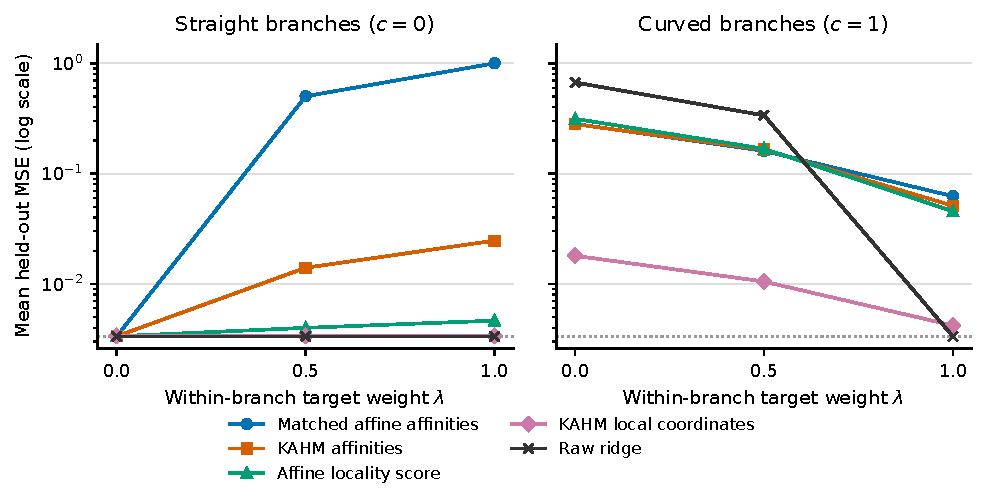
\includegraphics[width=.97\textwidth]{generated/figures/branch_alignment.pdf}
 \caption{Target relevance changes while branch inputs, fitted banks, and
 noise samples are held fixed within a repetition. The score-only affine
 code performs poorly when signed position matters on straight branches.
 Explicit local coordinates and a locality-aware affine scoring control
 remove most of the gap. The dotted line is the Bayes MSE $1/300$.
 The displayed mean errors summarize 24 repetitions;
 only the declared contrasts in the text belong to the primary interval family.}
 \label{fig:branch}
\end{figure}

\begin{table}[t]
 \caption{The six primary branch settings at 1,024 training points:
 mean ridge test MSE over 24 repetitions, with the primary KAHM advantage
 $G$ and its interval from the 29-comparison family. The Bayes MSE is
 $1/300$. The affine-locality scoring control reuses the shared references
 and is secondary.}
 \label{tab:branch}
 \centering\small\setlength{\tabcolsep}{3pt}
 % Generated by scripts/build_paper_assets.py; do not edit.
\begin{tabular}{rrrrrl}
\toprule
$c$ & $\lambda$ & Affine $\phi$ & KAHM $\phi$ & Affine locality & $G$ [interval] \\
\midrule
0 & 0 & 0.003334 & 0.003347 & 0.003344 & $-0.000013\;[-0.000031,\,0.000005]$ \\
0 & 0.5 & 0.503448 & 0.013995 & 0.003991 & $0.489453\;[0.481962,\,0.496944]$ \\
0 & 1 & 1.002694 & 0.024668 & 0.004641 & $0.978026\;[0.962552,\,0.993500]$ \\
1 & 0 & 0.282887 & 0.281126 & 0.314394 & $0.001761\;[-0.071260,\,0.074781]$ \\
1 & 0.5 & 0.160813 & 0.165207 & 0.167971 & $-0.004395\;[-0.043672,\,0.034882]$ \\
1 & 1 & 0.062366 & 0.051042 & 0.045555 & $0.011324\;[0.000882,\,0.021767]$ \\
\bottomrule
\end{tabular}

\end{table}

The scoring controls are essential to interpreting the large contrast.
A locality-aware affine score gives mean error \FlatWithinNativeAffineMSE{}, and affine local
coordinates give 0.00333, close to the Bayes error and raw ridge. Therefore,
the large advantage over matched affine affinities is not evidence that
affine geometry is intrinsically unable to predict this target. It is
evidence that a residual-based encoding can discard positional information
and that KAHM's induced score variation can retain it. An explicit
position-preserving code achieves the same practical purpose more directly.

The primary target interaction also constrains the interpretation. On
straight branches, $G(\lambda=0)-G(\lambda=1)=\FlatAlignmentInteraction$, with simultaneous
interval $[-0.99351,-0.96257]$. The KAHM advantage is greater when signed
position matters, rather than when branch identity alone matters. The
corresponding curved-branch interaction is unresolved. These results
disfavor a simple account in which the useful KAHM property is merely
separation of branch regimes. The native-score controls support the more
specific positional interpretation, although those controls were not members
of the formal interaction contrast.

\subsection{Local coordinates repair a predictive bottleneck, without making it KAHM-specific}
\label{sec:localresults}

Adding gated local coordinates to KAHM affinities improves ridge prediction
in \LocalPracticalBenefitCount{} of the nine primary settings. In all eight, the simultaneous
interval clears the prespecified practical margin. The exception is the
straight-branch, identity-only target, where the small adverse difference
is below that margin in magnitude. Adding $\log Z$ improves seven settings
under the primary intervals, five by more than their practical margins.
Neither intervention is a universal improvement.

The three forecasting laws show the scale of the local-coordinate effect
(Table~\ref{tab:ridge}). On Van der Pol, KAHM ridge MSE falls from \VDPPhiRidgeMSE{}
to \VDPKAHMLocalRidgeMSE{}; on Duffing it falls from 0.05373 to 0.00756. However, affine
local features are still better under ridge on both laws. The first-stage
geometry contrasts alone therefore do not establish a KAHM advantage on
the oscillators. They establish that score-only KAHM codes are an
inadequate predictive interface for these restricted heads.

\begin{table}[t]
 \caption{All nine first-stage primary settings: mean test MSE over
 24 repetitions for ridge decoders. The local-coordinate improvement $L$
 and its interval belong to the 29-comparison family. Retaining local
 position substantially improves KAHM prediction in eight settings;
 KAHM local coordinates do not dominate affine local coordinates.}
 \label{tab:ridge}
 \centering\small\setlength{\tabcolsep}{3pt}
 % Generated by scripts/build_paper_assets.py; do not edit.
\begin{tabular}{lrrrrl}
\toprule
Setting & KAHM $\phi$ & KAHM local & Affine local & Raw & $L$ [interval] \\
\midrule
$c=0,\lambda=0$ & 0.003347 & 0.003378 & 0.003337 & 0.003338 & $-0.000031\;[-0.000043,\,-0.000020]$ \\
$c=0,\lambda=0.5$ & 0.013995 & 0.003379 & 0.003333 & 0.003334 & $0.010616\;[0.010033,\,0.011200]$ \\
$c=0,\lambda=1$ & 0.024668 & 0.003380 & 0.003333 & 0.003330 & $0.021287\;[0.020199,\,0.022376]$ \\
$c=1,\lambda=0$ & 0.281126 & 0.017982 & 0.048916 & 0.671776 & $0.263144\;[0.217187,\,0.309101]$ \\
$c=1,\lambda=0.5$ & 0.165207 & 0.010497 & 0.026756 & 0.337620 & $0.154710\;[0.122867,\,0.186552]$ \\
$c=1,\lambda=1$ & 0.051042 & 0.004188 & 0.004656 & 0.003329 & $0.046854\;[0.040400,\,0.053307]$ \\
Nonlinear AR & 0.005300 & 0.004867 & 0.004867 & 0.005053 & $0.000433\;[0.000368,\,0.000498]$ \\
Van der Pol & 0.111108 & 0.014475 & 0.011582 & 0.041340 & $0.096633\;[0.092436,\,0.100830]$ \\
Duffing & 0.053729 & 0.007560 & 0.004448 & 0.006764 & $0.046168\;[0.041729,\,0.050608]$ \\
\bottomrule
\end{tabular}

\end{table}

The inverse in Equation~\eqref{eq:inverse} is verified numerically with
maximum error about $2.8\times10^{-16}$ on the checked representations.
Even so, the first-stage Van der Pol KAHM-score RBF error is 0.00158,
whereas the information-equivalent $[\phi,\log Z]$ RBF error is 0.01273.
This secondary comparison illustrates that preserving information does
not equalize access to it under a particular finite decoder and tuning
scheme. It also cautions against interpreting every local-coordinate gain
as a proof of irreversible information loss in the original representation.

\subsection{Fresh data confirm a conditional KAHM forecasting advantage}
\label{sec:capacity}

Table~\ref{tab:capacity} reports the second-stage comparison. On Van der Pol,
KAHM local-coordinate features outperform both alternatives at 64 and 256
landmarks in all 24 repetitions. At 256 landmarks, mean MSE is \VDPKAHMWideMSE{}
for KAHM local coordinates, \VDPAffineWideMSE{} for affine local coordinates, and
\VDPRawWideMSE{} for raw histories. The corresponding relative reductions,
computed from the means, are \VDPAffineWideRelativeGain\% and \VDPRawWideRelativeGain\%. These percentages are
descriptive ratios; the primary inferential quantities are paired absolute
differences.

At 256 landmarks, the simultaneous lower endpoints of the raw-minus-KAHM
and affine-minus-KAHM intervals are $0.00075496$ and $0.00018100$,
respectively (Table~\ref{tab:capacity}). Both exceed the frozen practical
margin $0.00014891$. The two corresponding
64-landmark intervals also clear that margin. Thus the positive result
survives the tested increase in nonlinear decoder budget. Increasing the
budget improves raw and affine performance too; this is not evidence of an
asymptotic separation between representation families.

\begin{table}[t]
 \caption{Fresh second-stage forecasting results: mean MSE over 24 new
 repetitions per law, with $M=64$ or $256$ RBF landmarks. All MSEs,
 differences, and interval endpoints are multiplied by $10^3$.
 The difference $\Delta$ is control minus KAHM-local MSE; positive favors
 KAHM. Intervals belong to the separate 12-comparison family. The same
 decoder family and tuning grid are used, with gains on Van der Pol
 and losses on the other laws.}
 \label{tab:capacity}
 \centering\small\setlength{\tabcolsep}{3pt}
 % Generated by scripts/build_paper_assets.py; do not edit.
\begin{tabular}{lrlrrl}
\toprule
System & $M$ & Control & Control MSE & KAHM local MSE & $\Delta$ [interval] \\
\midrule
Nonlinear AR & 64 & Raw & 4.4238 & 4.8795 & $-0.4556\;[-0.5235,\,-0.3878]$ \\
Nonlinear AR & 64 & Affine local & 4.9120 & 4.8795 & $0.0325\;[-0.0031,\,0.0680]$ \\
Nonlinear AR & 256 & Raw & 4.6958 & 5.1749 & $-0.4791\;[-0.6013,\,-0.3569]$ \\
Nonlinear AR & 256 & Affine local & 5.2347 & 5.1749 & $0.0598\;[-0.0131,\,0.1327]$ \\
\midrule
Van der Pol & 64 & Raw & 2.8586 & 1.0266 & $1.8320\;[1.7369,\,1.9271]$ \\
Van der Pol & 64 & Affine local & 1.3767 & 1.0266 & $0.3501\;[0.2755,\,0.4247]$ \\
Van der Pol & 256 & Raw & 1.6541 & 0.8720 & $0.7822\;[0.7550,\,0.8094]$ \\
Van der Pol & 256 & Affine local & 1.0780 & 0.8720 & $0.2060\;[0.1810,\,0.2311]$ \\
\midrule
Duffing & 64 & Raw & 3.4597 & 4.2154 & $-0.7557\;[-1.0831,\,-0.4282]$ \\
Duffing & 64 & Affine local & 3.0549 & 4.2154 & $-1.1605\;[-1.4707,\,-0.8503]$ \\
Duffing & 256 & Raw & 2.8364 & 4.0736 & $-1.2372\;[-1.5242,\,-0.9503]$ \\
Duffing & 256 & Affine local & 2.7981 & 4.0736 & $-1.2756\;[-1.5702,\,-0.9810]$ \\
\bottomrule
\end{tabular}

\end{table}

\begin{figure}[t]
 \centering
 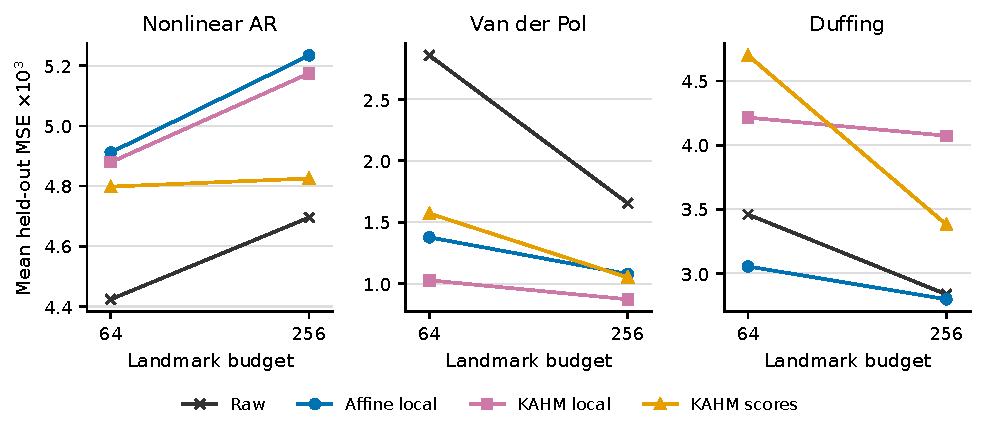
\includegraphics[width=.98\textwidth]{generated/figures/forecast_capacity.pdf}
 \caption{Mean second-stage forecasting errors as the nominal nonlinear
 decoder budget increases. Feature dimensions and effective Nystr\"om ranks
 differ, so the horizontal axis is a landmark budget rather than an exactly
 equalized model capacity. The ordering depends on the forecasting law.}
 \label{fig:forecast}
\end{figure}

The adverse comparisons matter for the scope of the result. On nonlinear
AR, raw histories outperform KAHM local features at both widths; the
KAHM--affine differences are unresolved. On Duffing, both raw and affine
local features outperform KAHM local features at both widths. At 256
landmarks, mean Duffing MSE is about 0.002798 for affine local features and
0.004074 for KAHM local features. All four corresponding adverse
raw/affine comparisons have simultaneous intervals excluding zero.
The advantage therefore does not follow from the label ``nonlinear
oscillator'' alone.

\begin{figure}[t]
 \centering
 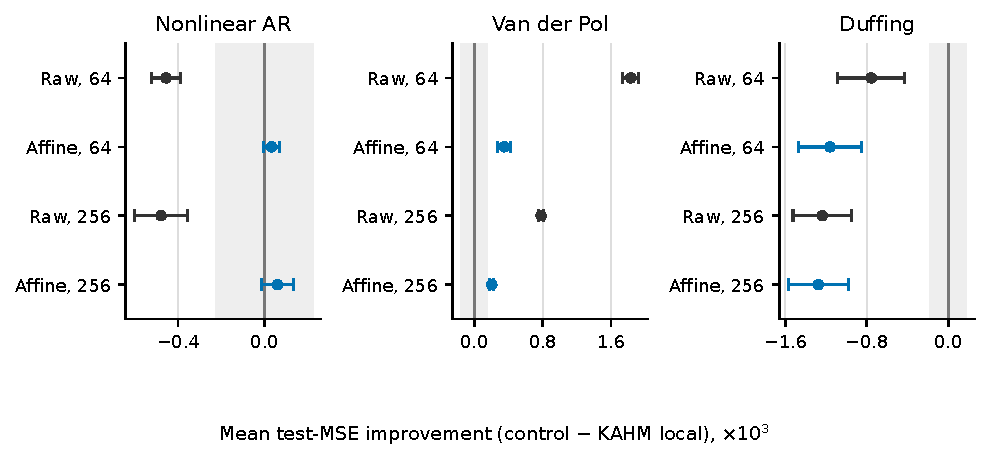
\includegraphics[width=.98\textwidth]{generated/figures/capacity_contrasts.pdf}
 \caption{All 12 primary second-stage contrasts, each defined as comparator
 MSE minus KAHM-local MSE. Positive values favor KAHM. Intervals use the
 second-stage 95\% Bonferroni family across 24 paired full data-and-fit
 repetitions. Gray bands mark the fixed $\pm$ practical margins from
 first-stage raw-RBF errors. This family
 is separate from the 29 first-stage contrasts.}
 \label{fig:contrasts}
\end{figure}

These results establish the utility of the declared KAHM pipeline on the
specified Van der Pol law and sampling design. They do not establish a
task-independent geometric statistic that predicts the advantage. In
particular, the straight-branch reflection experiment does not prove that
the same symmetry explains Van der Pol. Connecting an independently
measured geometric diagnostic to a held-out task's KAHM advantage is a
remaining research problem.

\subsection{Gaussian query underflow does not explain the local-feature advantage}
\label{sec:numerical}

The original query kernel can underflow when every Gaussian value in a
query row becomes numerically zero. Because the kernel weights are
normalized, multiplying a nonzero row by a common positive constant
does not change the exact reconstruction. We therefore performed a
post-hoc sensitivity analysis using the stable evaluation
\begin{equation}\label{eq:stable}
 \widetilde{k}_{cj}(z)=
       \exp\{\ell_{cj}(z)-\max_i\ell_{ci}(z)\},
 \qquad
 \ell_{cj}(z)=-\frac{\Delta_{cj}(z)^\top\Sigma_c^{-1}\Delta_{cj}(z)}{2p_c},
\end{equation}
where $\Delta_{cj}(z)=P_c^\top(z-v_{cj})$, $v_{cj}$ is reference $j$,
$p_c$ is the retained local rank, and $\Sigma_c$ is the projected reference
covariance. We compute $\ell_{cj}$ directly from this quadratic form,
before exponentiation; taking logarithms of already underflowed kernel
values would not repair an all-zero row. We keep the fitted references,
basis, regularized matrix, and data
unchanged. We refitted and validation-tuned the affected heads consistently
under this query evaluation. This is a robustness analysis on reused
second-stage Van der Pol data, not an additional independent confirmation.

Across \NumericalQueryClusterCount{} test query--local-model evaluations, the
original implementation has \NumericalOriginalZeroCount{} exactly zero weight normalizers; the stable
evaluation has none. Despite this substantial numerical diagnostic,
mean KAHM-local test MSE changes by less than $4\times10^{-13}$ at either
width. Its advantage over raw and affine local features remains positive
in all 24 repetitions at both widths. Full-score features change more:
their mean errors improve by approximately 0.37--0.39\%, and some
individual predictions change appreciably. We therefore do not claim that
the numerical issue is irrelevant to every representation.

\begin{table}[t]
 \caption{Post-hoc Van der Pol numerical sensitivity on the same 24
 second-stage banks and samples. Stable query evaluation removes observed
 zero denominators while leaving local-coordinate mean MSE effectively
 unchanged. $\Delta_r$ is the original-minus-stable MSE difference within
 repetition $r$; wins count stable predictions beating the raw and affine
 local controls at the same width. These comparisons are outside the two primary
 interval families.}
 \label{tab:numerical}
 \centering\small
 % Generated by scripts/build_paper_assets.py; do not edit.
\begin{tabular}{lrrrrl}
\toprule
Encoding & $M$ & Original MSE & Stable MSE & Max. $|\Delta_r|$ & Wins raw; affine \\
\midrule
Local & 64 & 0.001026627 & 0.001026627 & $1.01\times10^{-12}$ & 24/24; 24/24 \\
Local & 256 & 0.000871969 & 0.000871969 & $1.69\times10^{-11}$ & 24/24; 24/24 \\
Scores & 64 & 0.001571085 & 0.001565219 & $8.74\times10^{-5}$ & 24/24; 4/24 \\
Scores & 256 & 0.001049909 & 0.001045801 & $3.53\times10^{-5}$ & 24/24; 17/24 \\
\bottomrule
\end{tabular}

\end{table}

The practical implication is to stabilize the inner kernel evaluation and
retain explicit diagnostics for near-zero or cancelling signed normalizers.
Row scaling handles Gaussian underflow; it does not guarantee that signed
weights can never cancel. The archived main results retain the original
implementation so that the sensitivity comparison remains inspectable.

\subsection{A natural-data check limits claims of general predictive superiority}
\label{sec:airfoil}

The secondary Airfoil experiment favors the raw RBF predictor
(Table~\ref{tab:airfoil}). Its mean group-weighted MSE is \AirfoilRawRBFMSE\,dB$^2$,
compared with \AirfoilRawRidgeMSE{} for raw ridge, 20.90 for KAHM local-coordinate ridge,
31.86 for KAHM affinity ridge, and 34.16 for affine affinity ridge.
The first-stage validation selector chooses raw RBF in all 24 fits.
This is evidence against treating the KAHM construction as a default
replacement for raw-input regression. Because all seeds share the same
held-out operating-condition groups, their spread is not an uncertainty
interval for generalization to arbitrary natural datasets or new group
populations.

\begin{table}[t]
 \caption{Secondary Airfoil static-regression results on one fixed group
 split, averaged over 24 fitting seeds. Units are dB$^2$. These seeds do
 not constitute independent natural-data replications, and the comparison
 is descriptive.}
 \label{tab:airfoil}
 \centering\small
 % Generated by scripts/build_paper_assets.py; do not edit.
\begin{tabular}{lrr}
\toprule
Representation & Ridge MSE & RBF$_{64}$ MSE \\
\midrule
Raw & 19.4726 & 15.6898 \\
Affine $\phi$ & 34.1630 & 36.0476 \\
KAHM $\phi$ & 31.8586 & 34.3338 \\
Affine local & 22.7200 & 22.4050 \\
KAHM local & 20.9040 & 20.9313 \\
KAHM scores & 24.2168 & 21.7070 \\
\bottomrule
\end{tabular}

\end{table}

\section{How the Findings Change the Model}\label{sec:implications}

\subsection{Retain local position at the predictive interface}

The first change is to expose local position instead of making every
predictor rely on normalized reconstruction scores alone. Equation~\eqref{eq:local}
is a compact implementation of that change. It retains the interpretation
of affinities as local gates while giving the decoder coordinates that
vary within a local region. The branch intervention and the eight positive
local-coordinate contrasts support this change for the studied settings.
The affine control shows that it is a general representation principle
whose usefulness should not be attributed solely to KAHM reconstruction.

Retaining $\log Z$ is a different intervention: it recovers the score vector's
absolute scale in exact arithmetic, but does not directly expose position.
The two augmentations should therefore not be treated as interchangeable.
Full scores and raw-input skips are useful controls when a score-based
predictor underperforms, because they test different possible bottlenecks.

\subsection{Select the representation together with its decoder}

The second change is to evaluate a complete representation--decoder pair.
The first-stage ridge ordering would miss the favorable Van der Pol
KAHM-local result available to the nonlinear head. Conversely, the existence
of that favorable pair does not justify choosing it on Duffing or AR.
The implemented second-stage selector considers the eight combinations
of four representations and two landmark widths. Each candidate's
hyperparameters are selected by validation, and the candidate with the
lowest validation MSE supplies the final prediction. Test data play no
role in either decision. This protocol was specified before the fresh
second-stage data were generated.

The selector chooses raw inputs with 64 landmarks in all 24 AR repetitions,
KAHM local coordinates with 256 landmarks in all 24 Van der Pol repetitions,
and affine local coordinates with 256 landmarks in 23 of the 24 Duffing
repetitions; the remaining Duffing choice is raw input with 256 landmarks.
Mean selector errors are approximately 0.004424, 0.000872, and 0.002792,
respectively. These are secondary operational results for the declared
candidate set, not an oracle comparison with all learning algorithms.
Selection adds validation use and computational cost, and a new task can
require a larger or differently designed validation set
\citep{Cawley2010Selection}.

The companion implementation exposes \texttt{PredictiveGeometryRegressor}
with training and validation inputs, optional validation groups, prediction,
and state serialization. Its default candidate family reproduces this
selector. A raw-input selection avoids geometric queries at prediction
time. The reusable wrapper was assembled after the experiments, and its
predictions were checked against the archived selection procedure; its
existence does not constitute an additional experiment.

\subsection{Use reconstruction as a diagnostic, not the sole selection objective}

The third change is evaluative. A geometric model should report how its
code treats target-relevant variation alongside input reconstruction.
On a controlled distribution this can be done using a known conditional
mean, a target intervention, or a distribution-preserving transformation.
On an unknown task, a fitted target predictor can provide an exploratory
diagnostic, but its errors and selection must be accounted for before
using it to claim an information-loss certificate.

For KAHM development, a useful next objective is therefore to learn or
select local gates for predictive performance while retaining direct local
coordinates and a raw-input alternative. We have implemented validation
selection among fixed candidates; we have not tested a new supervised
training objective for the KAHM reconstruction bank. Such an objective is
a consequence to investigate, rather than a result established here.

\section{Scope, Limitations, and Research Direction}\label{sec:limits}

The positive evidence has a specific scope. It concerns the declared
generators, training and validation sizes, observation maps, horizons,
small local bank, feature scaling, decoder grids, and test distributions.
The capacity follow-up guards against a favorable first-stage seed outcome
and checks two finite budgets. It does not remove task-selection effects:
Van der Pol was a promising setting observed in the first stage, and we
explicitly used that observation to motivate the follow-up. The other two
laws were retained to test the breadth of the finding.

The controlled comparison changes one reconstruction rule inside a matched
construction. This supports component attribution, but it does not establish
superiority over independently optimized affine local learning. Indeed,
the locality-aware affine scoring control nearly closes the straight-branch
gap. Local-coordinate augmentation also changes dimensionality and
regularization geometry. Its gain cannot be assigned wholly to information
recovery, and an equal nominal landmark count is not an exactly equal
number of effective parameters. At 256 landmarks on Van der Pol, for
example, the retained RBF-plus-linear dimensions are 268 for raw inputs,
298 for affine local coordinates, and approximately 272 on average for
KAHM local coordinates after the eigenvalue cutoff.
Table~\ref{tab:capacity-dimensions-details} reports the retained dimensions
for all laws, representations, and landmark budgets.

The statistical analysis uses paired $t$ approximations across independent
synthetic repetitions. Bonferroni adjustment protects the declared family
only to the extent that these marginal approximations are adequate.
The intervals do not cover every exploratory analysis. Runtime measurements
share intermediate computations across methods and are not fair standalone
end-to-end speed comparisons. The numerical sensitivity exercise addresses
one concrete implementation risk on reused Van der Pol data; it is not a
complete conditioning analysis of signed kernel normalization.

The natural-data evidence is narrow and adverse for the presented KAHM
variants. A broader claim about machine learning utility requires natural
forecasting datasets, strong raw-input and local-model baselines, and
protocols that respect series or subject boundaries. We have not compared
against a modern, broadly tuned forecasting suite or demonstrated
state-of-the-art forecasting. The present contribution is an explanatory
and reproducible study of a particular geometric model family.

Most importantly, there is not yet a validated diagnostic that predicts
before fitting the downstream model when KAHM geometry will help on a
new task. A credible next test would define such a diagnostic using
training and validation data, freeze its prediction of relative benefit,
and evaluate that prediction across held-out tasks. Candidate quantities
include target-relevant changes along local directions and the sensitivity
needed to decode the corresponding code, rather than reconstruction
error alone. The test must include tasks with different observation maps,
noise levels, sample sizes, and dynamics, and must retain cases where
the prediction is wrong. This would convert a conditional empirical
finding into transferable model-selection knowledge.

\section{Conclusion}

KAHM geometry can help prediction, but its benefit depends on what the
predictive representation retains and which decoder uses it. In a
controlled branch experiment, KAHM-derived scores preserve signed
positional variation that a matched affine residual code nearly removes,
despite worse reconstruction. Explicit local coordinates expose that
variation for both geometries. In a separately designed fresh-sample
forecasting study, KAHM local coordinates with a finite nonlinear decoder
give a clear advantage on Van der Pol and lose on other declared laws.
The resulting model design retains local position, allows decoder
flexibility, and selects among geometric and raw-input alternatives using
validation data. These findings support a precise development path for
KAHMs: study and exploit target-relevant geometry, while testing the
conditions of its advantage explicitly.

\section*{Code, Data, and Research Transparency}

The accompanying \path{TMLR_Reproducibility_Supplement.zip} contains the source snapshot, fixed
configurations and seed rules, compact historical results, statistical
audit scripts, paper-asset generators, and commands for fresh experiment
execution. Its reproduction guide distinguishes
historical-result verification, a small execution check, and a complete
regeneration. Fresh executions write separate output directories and
provenance; they do not overwrite or retrospectively recreate the
historical freezes. Generated model states and predictions support
loss recomputation and selected-model replay. Synthetic data are generated
from the specified laws. The included Airfoil data retain source,
checksum, and license attribution.

The KAHM routines are pinned to the upstream commit
\begin{center}\small\texttt{d6d74d1953a4310b73065a556df816e5ab5e3ebc}.\end{center}
The artifact records both
source hashes and the original numerical environment. Seeds and package
versions aid numerical reproduction but do not guarantee byte-identical
floating-point results across hardware and BLAS implementations. Timing
fields are not treated as deterministic scientific outcomes. Automated
checks compare the regenerated predictive quantities and primary contrasts
with the archived results within stated numerical tolerances.

\paragraph{Relationship to a related unpublished manuscript.}
\citet{Anonymous2026Certificates} studies risk certificates for
prescribed forecasting representation and decoder classes. The present
paper asks a different empirical question about KAHM geometry, encoding,
and finite fitted prediction. It uses shared upstream machinery and
generator definitions, but the target-intervention experiments, fresh
capacity follow-up, numerical sensitivity analysis, and validation-selected
model constitute the study reported here. The ridge and RBF heads are
not that manuscript's fixed sensitivity-budget classes, and no
certificate from that manuscript is transferred to these fitted results.
Anonymized copies are included as \path{Related_Manuscript.pdf} and
\path{Related_Manuscript_Supplement.pdf} in the accompanying supplementary
ZIP to support assessment of the relationship between the studies.

\paragraph{Use of AI tools.}
AI tools assisted with study implementation, numerical and statistical
checks, literature retrieval, reproducibility packaging, and manuscript
drafting. The executable artifact and recorded evidence are provided to
support independent scrutiny of the claims. The authors are responsible
for the manuscript's content and for checking the resulting claims.

\bibliographystyle{tmlr}
\bibliography{references}
\clearpage
\appendix
% Supporting theory and exact methods. The main document invokes \appendix.
\section{Supporting Mathematical Statements}\label{app:theory}

The statements in this appendix make the interpretation of the experiments
precise. They are elementary supporting results; we do not claim a new
KAHM approximation theorem. All conditional expectations below are understood
up to almost-sure equality. For scalar square-integrable $Y$, write
$m(X)=\E[Y\mid X]$ and
$R_X^{\mathrm{Bayes}}=\E[(Y-m(X))^2]$.
When a representation has been learned from independent training data,
the statements apply conditionally on that fitted representation.

\begin{proposition}[Information retained by a representation]
\label{prop:representation-risk}
For a measurable representation $U=\Gamma(X)$,
\[
 R_U^{\mathrm{Bayes}}-R_X^{\mathrm{Bayes}}
 =\E[(m(X)-\E[m(X)\mid U])^2].
\]
For any square-integrable prediction $f(U)$,
\[
 R(f\circ\Gamma)-R_X^{\mathrm{Bayes}}
 =\|m-f\circ\Gamma\|_{L^2}^2.
\]
\end{proposition}
\begin{proof}
Write $Y-f(U)=(Y-m(X))+(m(X)-f(U))$.
The cross term has expectation zero after conditioning on $X$.
Minimizing the second term over $U$-measurable predictions gives the
conditional expectation $\E[m(X)\mid U]$.
\end{proof}

\begin{proposition}[Restoring the outer score normalizer]
\label{prop:normalizer-inverse}
Let $T_1,\ldots,T_C\in[0,1]$, $\omega>0$, and $\tau>0$. Define
\[
 \ell_c=\omega\log(1-T_c+\tau),\qquad
 z=\log\sum_{j=1}^{C}\exp(\ell_j),\qquad
 \phi_c=\exp(\ell_c-z).
\]
Then $T$ and $(\phi,z)$ generate the same information in exact arithmetic,
and
\[
 T_c=1+\tau-\exp\{(\log\phi_c+z)/\omega\}.
\]
For multiple separately normalized blocks, one $z$ is required per block.
\end{proposition}
\begin{proof}
Strict positivity of $1-T_c+\tau$ implies $\phi_c>0$.
Hence $\log\phi_c+z=\ell_c$, which gives the inverse.
Both directions are measurable. Applying this argument to each block
gives the multiple-block statement.
\end{proof}

If scores are clipped before normalization, the inverse restores the
clipped scores. It does not restore discarded reconstruction vectors or
guarantee equal finite-head performance. In particular, the inverse is
nonlinear, so affine function classes on $T$ and on $(\phi,z)$ need not
coincide. This proposition concerns the outer association normalizer,
not the signed denominator in the KAHM reconstruction.

\begin{proposition}[A sufficient condition for an injective local code]
\label{prop:local-injectivity}
Fix a fitted bank with bases $P_c$ and centers $\mu_c$. Suppose its gates
are measurable and strictly positive, and let $A$ be the matrix obtained by vertically
stacking the matrices $P_c^\top$. If $A$ has full column rank $d$, then
\[
 z\longmapsto
 \left[\phi(z),\{\phi_c(z)P_c^\top(z-\mu_c)\}_c\right]
\]
is injective. In particular, this code and $z$ generate the same
information, and their Bayes risks agree for every square-integrable
target.
\end{proposition}
\begin{proof}
The code contains both $\phi_c(z)>0$ and its product with
$P_c^\top(z-\mu_c)$. Division and addition of the fixed vector
$P_c^\top\mu_c$ recover $P_c^\top z$ for every $c$. Stacking these
vectors gives $Az$. Full column rank gives the measurable inverse
$z=(A^\top A)^{-1}A^\top(Az)$. Conversely, the code is a measurable
function of $z$, so the generated information and Bayes risks agree.
\end{proof}

The gates in Equation~\eqref{eq:phi} are strictly positive in exact
arithmetic because $\tau>0$. The rank assumption is a sufficient
condition, not a necessary one: when $A$ is rank deficient, the gates
themselves may retain additional information. It must be checked for
each fitted bank. Very small gates and an ill-conditioned $A$ can make
the displayed inverse numerically unstable, and its existence does not
make it accessible to every finite decoder or fitting procedure.

\begin{proposition}[A score symmetry and its prediction consequence]
\label{prop:exact-symmetry}
Let $Q$ be orthogonal on a preprocessed input space. Suppose that each
group's reconstruction obeys $r_c(Qx)=Qr_c(x)$ and that $Q$ preserves
group identities. The radial--angular score in Section~\ref{sec:method},
its block affinities, and the block log normalizer are invariant under $Q$.

For the branch law in Equation~\eqref{eq:branch}, let
$Q(x_1,x_2)=(-x_1,x_2)$. Any representation $U=\Gamma(X)$ satisfying
$\Gamma(QX)=\Gamma(X)$ almost surely has
\[
 R_U^{\mathrm{Bayes}}
 =\frac{1}{300}+\lambda
  +(1-\lambda)\E[(S-\E[S\mid U])^2].
\]
Consequently $R_U^{\mathrm{Bayes}}\geq 1/300+\lambda$, with equality
when $U$ determines $S$.
\end{proposition}
\begin{proof}
Orthogonality preserves norms and inner products, including the zero-norm
convention for the angle. Equivariance therefore preserves each radial
and angular discrepancy, hence its combined score. Block normalization
and its log normalizer are deterministic functions of those scores.

For the branch law, replacing $T$ by $-T$ leaves the joint distribution
of $(S,T)$ unchanged and leaves $U$ unchanged. Thus $\E[T\mid U]=0$.
Also $S$ is even under this reflection, whereas $T$ is odd. It follows
that $\E[(S-\E[S\mid U])T]=0$. Expanding the square in
Proposition~\ref{prop:representation-risk}, using
$\E[T^2]=1/3$ and $\Var(\epsilon)=1/300$, yields the displayed identity.
\end{proof}

The first assertion also holds when $Q$ permutes reconstructors within a
group whose score is their minimum. Permuting distinct groups, however,
can permute the affinity coordinates rather than leaving the representation
unchanged. Nor does a raw-input reflection necessarily commute with a
training-fitted scaler. Finite learned partitions and reference sets need
not satisfy the proposition's assumptions. The measured near-invariance
of one learned code is therefore a diagnostic, not a proof that its
Bayes risk equals the exact-symmetry lower bound. Tiny nonzero differences
could in principle be used by an unrestricted decoder.

\begin{proposition}[Approximate symmetry under a decoder budget]
\label{prop:approx-symmetry}
Let $Q$ be a measurable, distribution-preserving involution on the input
space: $Q^2X=X$ almost surely and $QX$ has the law of $X$.
Let $d_U$ be a measurable pseudometric on the representation space and
$g$ be $\kappa$-Lipschitz for this pseudometric. Assume
$m,g\circ\Gamma\in L^2$ and
\[
 \delta_\Gamma^2
 =\E[d_U(\Gamma(X),\Gamma(QX))^2]<\infty.
\]
With $m_o=(m-m\circ Q)/2$,
\[
 R(g\circ\Gamma)-R_X^{\mathrm{Bayes}}
 \geq (\|m_o\|_{L^2}-\kappa\delta_\Gamma/2)_+^2.
\]
For the branch law, $\|m_o\|_{L^2}=\sqrt\lambda$.
\end{proposition}
\begin{proof}
The operator $Vh=h\circ Q$ is an isometric involution on $L^2(P_X)$.
The even and odd components $h_e=(h+Vh)/2$ and $h_o=(h-Vh)/2$
are orthogonal. In particular, with $f=g\circ\Gamma$,
\[
 \|m-f\|_{L^2}^2
 =\|m_e-f_e\|_{L^2}^2+\|m_o-f_o\|_{L^2}^2
 \geq\|m_o-f_o\|_{L^2}^2.
\]
The Lipschitz condition gives
$|f_o(X)|\leq\kappa d_U(\Gamma(X),\Gamma(QX))/2$, so
$\|f_o\|_{L^2}\leq\kappa\delta_\Gamma/2$.
Apply the reverse triangle inequality and
Proposition~\ref{prop:representation-risk}.
For the branch law, $m_o(X)=\sqrt{3\lambda}\,T$ and
$\E[T^2]=1/3$.
\end{proof}

An empirical reflection distance is not automatically a population upper
bound for $\delta_\Gamma$. A valid numerical lower bound obtained from
this proposition would need uncertainty control in that direction and a
verified decoder Lipschitz constant for the same metric. Neither is
asserted for the experiment's unconstrained diagnostic heads.

\begin{proposition}[Reconstruction through the predictor's representation]
\label{prop:reconstruction-bridge}
Suppose a version of $m$ is $L$-Lipschitz on a domain containing $X$ and
$h(U)$ almost surely, and
$\E\|X-h(U)\|_2^2\leq\varepsilon_{\mathrm{rec}}^2$.
Then
\[
 R_U^{\mathrm{Bayes}}-R_X^{\mathrm{Bayes}}
 \leq L^2\varepsilon_{\mathrm{rec}}^2.
\]
If $h$ is additionally $L_h$-Lipschitz from the declared representation
metric and $\kappa\geq LL_h$, the same upper bound applies to the
infimum excess risk over $\kappa$-Lipschitz decoders:
\[
 \inf_{\operatorname{Lip}(g)\leq\kappa}
 \{R(g\circ\Gamma)-R_X^{\mathrm{Bayes}}\}
 \leq L^2\varepsilon_{\mathrm{rec}}^2.
\]
If a particular decoder
$f$ instead satisfies
$\|m\circ h-f\|_{L^2(P_U)}\leq\delta_{\mathrm{head}}$, then
\[
 R(f\circ\Gamma)-R_X^{\mathrm{Bayes}}
 \leq (L\varepsilon_{\mathrm{rec}}+\delta_{\mathrm{head}})^2.
\]
\end{proposition}
\begin{proof}
Conditional expectation is the $L^2$ projection onto the
$U$-measurable functions. The admissible prediction $m(h(U))$ gives
\[
 \E[(m(X)-\E[m(X)\mid U])^2]
 \leq \E[(m(X)-m(h(U)))^2]
 \leq L^2\E\|X-h(U)\|_2^2.
\]
For the constrained statement, $m\circ h$ has Lipschitz constant at
most $LL_h$. For a particular $f$, the triangle inequality in $L^2$
gives $\|m-f\circ\Gamma\|_{L^2}
\leq L\varepsilon_{\mathrm{rec}}+\delta_{\mathrm{head}}$.
Use Proposition~\ref{prop:representation-risk} in each case.
\end{proof}

The essential assumption is the existence of $h$ as a function of the
retained representation. A KAHM reconstruction evaluated on the raw query
is not such a function merely because its residual is small. The domain
assumption also matters: a conditional mean initially defined only on the
support of $X$ must have the specified Lipschitz version at $h(U)$.

\begin{proposition}[Common scaling of an inner kernel row]
\label{prop:inner-scaling}
Let $k$ be a finite kernel row, let $B$ be the fixed fitted matrix, and
suppose $kB\boldsymbol 1\ne0$. For every real $a>0$,
\[
 \frac{akB}{akB\boldsymbol 1}
 =\frac{kB}{kB\boldsymbol 1}.
\]
Thus evaluating a Gaussian query row by
$\exp(\ell_j-\max_i\ell_i)$ preserves its normalized signed weights
in exact arithmetic whenever the original denominator is nonzero.
\end{proposition}
\begin{proof}
The common factor cancels from numerator and denominator.
For finite log-kernel values, the centered exponential row is the
original row times $a=\exp(-\max_i\ell_i)>0$ in real arithmetic.
\end{proof}

This statement neither rescales the training kernel nor permits replacing
$B$. It does not address a genuinely zero signed denominator or prevent
cancellation. The purpose of the implemented change is to avoid evaluating
an entire query row as floating-point zero before normalization.

\section{Generators, Shared Components, and Decoders}\label{app:methods}

\subsection{Exact forecasting laws and target construction}

The nonlinear AR generator starts with independent
$u_0,u_1\sim\mathrm{Unif}[-0.8,0.8]$ and uses
\[
 u_{t+1}=\tanh\{1.25u_t-0.65u_{t-1}
                   +0.25\sin(3u_t)+\eta_{t+1}\},
 \qquad\eta_t\stackrel{\mathrm{iid}}\sim\mathrm{Unif}[-0.1,0.1].
\]
The first 80 stored values are discarded; the next 72 are the episode.
Each episode uses an independent initial state and innovation sequence.

The Van der Pol and Duffing systems respectively use
\begin{align*}
 \dot x&=v,& \dot v&=(1-x^2)v-x,\\
 \dot x&=v,& \dot v&=-0.2v+x-x^3+0.3\cos(1.2t+\theta).
\end{align*}
Initial positions and velocities are independent
$\mathrm{Unif}[-2,2]$ draws for each episode, and
$\theta\sim\mathrm{Unif}[0,2\pi]$ is independently sampled for each
episode. The phase draw is unused for Van der Pol but is retained in
the common generator's random-stream order. Both systems are integrated
using float64 classical fourth-order Runge--Kutta with step $0.025$,
burn-in time 10, and observation interval $0.1$. At the 72 observation
times, the sensor is
\[
 u_t=0.95\tanh(x_t)+\eta_t,
 \qquad \eta_t\stackrel{\mathrm{iid}}\sim\mathrm{Unif}[-0.02,0.02].
\]
Sensor noise is sampled before numerical integration in the frozen
generator. These define numerical data laws. We do not treat the
resulting samples as exact solutions of the continuous equations or
assume stationarity after burn-in.

For all three laws, zero-based forecast origins are
$11,15,\ldots,59$. At origin $t$, the input is
$(u_{t-11},\ldots,u_t)$ and the three targets are
$(u_{t+1},u_{t+4},u_{t+12})$. There are 13 origins per episode.
Training, validation, and test contain respectively 128, 128, and 512
independently generated episodes. They therefore contain 1,664, 1,664,
and 6,656 rows, but rows within an episode are dependent.

The branch law is Equation~\eqref{eq:branch}. Training has 1,024 points
for the primary study, with the first 256 points giving the secondary
nested sample-size condition. Validation and test have 512 and 2,048
independent points. At each repetition, the same latent draws of
$S,T,\epsilon$ generate both curvatures; within each curvature and
training size, one fitted bank serves all three target mixtures.
Latent labels never train the partitions. Since $T=X_1$ and
$S=2\{X_2-c\cos(\pi X_1)\}$, the raw inputs determine the signal.
Its variance is $(1-\lambda)+3\lambda/3=1$, and the independent
noise variance is $1/300$. The support bound
$|Y|\leq\sqrt{1-\lambda}+\sqrt{3\lambda}+0.1\leq2.1$
justifies the common clipping range.

The master random seed is 20261030. Separate phase identifiers and
child streams determine pilot, first confirmation, natural fitting,
and fresh capacity inputs and fits. The capacity phase identifier is
4. The archive contains the executable stream rules and the realized
identifiers. Reusing a replicate label across phases does not reuse its
observations. Common randomness within a repetition supports pairing;
it does not create additional independent repetitions.

\subsection{Training the common bank and defining the locality control}

The input mean and population-standard-deviation convention
($1/n$ variance divisor) are fitted on all training rows. A standard
deviation at most $10^{-12}$ is replaced by one. At most 1,600 training
rows, sampled without replacement, are used for clustering and
reference selection. Each of the three independent $k$-means block
fits uses five initializations and at most 150 iterations. Its
cluster counts are 2, 4, and 8. At most 24 reference rows per cluster
are sampled without replacement and converted to float32 before
the unchanged upstream autoencoder is called. The effective requested
rank is $\min(2,d-1,n_c-1)$, subject to upstream numerical rank
determination. The common reference mean and the resulting upstream
principal basis define the affine control.

For completeness, the pinned local KAHM fit can be written as follows.
Let $H\in\R^{d\times n_c}$ contain the float32 reference columns,
and set $q_i=P_c^\top H_i$. The basis is obtained from the centered
reference covariance with divisor $n_c-1$, retaining eigenvalues
above machine epsilon. The requested rank is reduced if a retained
projected coordinate has range below $10^{-3}$, until that condition
is removed or rank one is reached. With effective rank $r_c$ and
unbiased projected covariance $\Sigma_c$, the training kernel is
\[
 K_{ij}=\exp\left\{-\frac{(q_i-q_j)^\top\Sigma_c^{-1}(q_i-q_j)}{2r_c}\right\}.
\]
Writing $\nu=\|H\|_F^2/(dn_c)$, initialize $\rho_0=2.5\nu$ and iterate
\[
 B_j=(K+\rho_j I)^{-1},\qquad
 \rho_{j+1}=2\nu+
       \frac{\|H-H(KB_j)^\top\|_F^2}{dn_c}.
\]
The routine stops when $|\rho_{j+1}-\rho_j|\leq10^{-3}$ or after 100
iterations, returning the last computed $B_j$. This regularizer is
determined from reference inputs alone, independently of the supervised
target. Query kernels use the same projected covariance metric and
$1/(2r_c)$ Gaussian scale. A cluster with fewer than two usable
references or no positive empirical-variance direction has the recorded
center reconstruction fallback; other numerical failures are not
silently replaced by another method.

The two reconstruction methods have the same input basis but not
identical functional capacity. KAHM uses its nonlinear query weights
to combine full-dimensional reference vectors; it need not remain
inside the truncated affine PCA plane. A shared basis does not make
its reconstruction an affine projection. The experiment isolates the
reconstruction operator within the specified bank, not all possible
advantages of independently optimized complete systems.

The alternative affine locality score is essential to interpreting
the straight-branch comparison. In standardized input space, let
\begin{align*}
 s_c&=\max\left\{\frac1{n_c}\sum_{i\in c}\|z_i-\mu_c\|_2^2,10^{-6}\right\},\\
 v_c&=\max\left\{\frac1{n_c}\sum_{i\in c}
       \|(I-P_cP_c^\top)(z_i-\mu_c)\|_2^2,
       0.05s_c,10^{-6}\right\}.
\end{align*}
It uses
\[
 b_c(z)=\frac{\|z-r_c^{\A}(z)\|_2^2}{v_c}
               +0.1\frac{\|z-\mu_c\|_2^2}{s_c},\qquad
 \psi_c(z)=\frac{\exp(-b_c(z))}{\sum_{j\text{ in block}}\exp(-b_j(z))}.
\]
This retains a center-distance term that distinguishes positions along
an otherwise exactly reconstructed line. It changes the scoring rule
and is a secondary control, not part of the primary reconstruction
substitution. A radial-basis locality control similarly normalizes
$\exp\{-\|z-\mu_c\|_2^2/(2\operatorname{median}_j s_j)\}$ within a block.

There are 14 stored affinity coordinates and three block-sum constraints,
giving an affine-dimension upper bound of 11 for the concatenated
affinities. Appending the three log normalizers gives 17 stored
coordinates. Local augmentation gives 28 coordinates for the
two-dimensional branches and 42 for the 12-dimensional forecasting
histories. The added coordinates are
$\phi_c P_c^\top(z-\mu_c)$, computed from the original query in the
shared basis; full reconstruction vectors are not passed to these heads.

For reconstruction diagnostics, each query's squared reconstruction
distance is divided by input dimension. The best-model diagnostic
takes the minimum across local models in each block; the weighted
diagnostic takes the sum with that reconstruction's own affinity weights.
Both then average across queries, blocks, and repetitions. Thus the
weighted summary is an affinity-weighted average of individual errors,
not the reconstruction error of the affinity-weighted vector. These
descriptive summaries are not additional primary forecast contrasts.

\subsection{Ridge and finite nonlinear heads}

Each input feature column is standardized using training data alone.
Standard deviations below $10^{-8}$ are replaced by one. The ridge
fit minimizes mean squared training error plus
$\alpha\|W\|_F^2$, with an unpenalized intercept. The fixed penalty
grid is
\[
 \alpha\in\{10^{-8},10^{-6},10^{-4},10^{-3},10^{-2},10^{-1},1\}.
\]
Validation chooses the penalty. Forecast horizons share that choice;
the three branch targets choose separately.

The nonlinear head first selects $M$ training rows without replacement
as landmarks in the standardized input-feature space. For a fixed
budget, the common seed selects the same row indices across the
representations, though their feature values differ. Let $b^2$ be the
median strictly positive squared landmark distance, excluding distances
at most $10^{-14}$; if no such distance exists, use $b^2=1$.
For bandwidth multiplier $a\in\{0.25,1,4\}$, the squared bandwidth is
$\max(b^2a^2,10^{-12})$. Form the Gaussian landmark matrix $K_{MM}$,
symmetrize it, and retain eigenvalues exceeding
$\max(10^{-10}\lambda_{\max},10^{-12})$. If
$K_{MM}=V\Lambda V^\top$ on the retained subspace, the nonlinear
coordinates are $K_{xM}V\Lambda^{-1/2}$. Concatenate these coordinates
with the standardized linear input features; standardize the full
resulting basis on training data and fit the same ridge objective.
Validation selects a bandwidth--penalty pair using the fixed nested
iteration order, so ties are deterministic. The first stage uses
$M=64$; the fresh follow-up uses both $64$ and $256$.

Because basis columns are standardized and assigned an ordinary Euclidean
ridge penalty, this is a finite nonlinear diagnostic with a linear
component. It is not an exact kernel-ridge estimator with its standard
RKHS norm. Effective dimension can be smaller than input dimension
plus $M$ after the eigenvalue cutoff. Increasing $M$ can change the
sampled landmark set, median-distance bandwidth, retained rank, and
validation-selected hyperparameters. It does not isolate only a
dimension parameter while holding the realized basis fixed.

Predictions are clipped to the known target range for both validation
and test evaluation, but the ridge objective itself is the un-clipped
training least-squares objective. The selected coefficients remain
fitted on training data; validation observations are not used in a
final combined fit. The secondary capacity selector chooses the lowest
validation MSE among the eight complete representation--budget pipelines.
Its fixed tie order is ascending budget followed by the configured
feature order. The test split chooses neither hyperparameters nor
the complete pipeline.

\subsection{Airfoil grouping and the scope of its repetitions}

The Airfoil snapshot contains 1,503 rows with five covariates and sound
pressure as the target. Exact joint equality of the four non-frequency
covariates defines 106 operating-setting groups. A fixed permutation
with seed 2026103007 allocates 64, 21, and 21 groups to training,
validation, and test, giving 905, 295, and 303 rows. All frequency rows
within a setting stay together. The training objective weights rows
equally; validation and test average within a group before weighting
groups equally. The outcomes are reported in squared decibels.

The 24 seeds repeat fitting on this same observed cohort and split.
They characterize fitting variability conditional on those data.
No primary synthetic-experiment interval is applied to Airfoil, and
the 24 fits are not treated as 24 independent draws of natural tasks,
test cohorts, or physical operating-condition populations. A population
claim would require a justified sampling model or independent cohorts.

\section{Estimands, Multiplicity, and Descriptive Diagnostics}\label{app:statistics}

\subsection{The unit of paired inference}

For forecast method $A$ and repetition $r$, the reported loss is
\[
 \widehat L_{r,A}=\frac1{512}\sum_{j=1}^{512}
      \frac1{13\cdot3}\sum_{o=1}^{13}\sum_{h\in\{1,4,12\}}
              (\widehat y_{r,A,j,o,h}-y_{r,j,o,h})^2.
\]
For branches it is the mean noisy-target squared error over 2,048
test points. The conditional-mean target loss is a separate secondary
diagnostic. Each method and target at a given repetition shares the
declared test draws, yielding a paired contrast. The independent units
for the primary intervals are the 24 complete train--validation--test
repetitions. Overlapping windows, horizons, reference groups, candidate
fits, and three target mixtures are not extra replication units.

For each primary paired contrast $D_r$, let $\overline D$ be its sample
mean and $s_D$ its unbiased sample standard deviation over 24 repetitions.
For family size $F$, the interval is
\[
 \overline D\ \mathbin{\pm}\
 t_{23,\,1-0.05/(2F)}\,\frac{s_D}{\sqrt{24}}.
\]
The critical values are approximately 3.545808 for $F=29$ and 3.180663
for $F=12$. Under independent normal paired differences, each marginal
Student interval has its exact nominal coverage, and the Bonferroni
union bound gives family coverage at least 95\%. Under other laws,
the Student coverage is approximate. Twenty-four repetitions do not
guarantee an adequate normal approximation. The results are not
distribution-free certificates. Dependence between contrasts is
allowed by Bonferroni; independence of windows is never used.

The synthetic estimand includes training and validation randomness,
as well as finite test-sample variation, under each declared numerical
generator. It is not an average over an independently sampled population
of forecasting tasks. The sample size of 24 was fixed as a resource
decision, not justified by an unreported prospective power calculation.

\subsection{Comparison families and practical margins}

The first-stage family contains the 27 $G,N,L$ contrasts over nine
settings and the two interactions
$I_c=G(c,\lambda=0)-G(c,\lambda=1)$. A positive interaction would
favor a larger reconstruction advantage for the branch-identity target.
Negative $I_c$ is the opposite direction of this hypothesis, not a
literal statement that one fitted method is uniformly harmful.
The cell margin is 5\% of the mean raw-ridge MSE from two pilot
repetitions. Each interaction margin is the mean of its two endpoint
cell margins. All pilot outcomes are excluded from confirmation
estimates. The margins are recorded design thresholds, not externally
validated application tolerances; their scale estimate has only two
pilot observations.

The fresh capacity family contains 12 differences: raw minus KAHM
local and affine local minus KAHM local, for three systems and two
budgets. Each law's margin is 5\% of its first-stage mean raw-RBF
MSE, using the complete 24 first-stage confirmation repetitions.
The margins, candidate list, and 24 fresh replication streams were
frozen before phase-4 data were generated. Conditional on the completed
first stage, they are fixed for this follow-up. The follow-up is
explicitly data-motivated; it is not retroactively part of the initial
29-comparison plan. Its separate 95\% family does not imply joint
95\% coverage with the first family.

We call a difference a practical benefit at the declared threshold
only when its simultaneous lower endpoint exceeds its fixed margin.
An interval strictly above zero but not above the margin establishes
a positive difference under the interval assumptions without resolving
that practical threshold. A negative interval indicates an adverse
difference for the candidate. An interval containing zero leaves the
direction unresolved. An interval entirely within the fixed band
$[-\delta,\delta]$ can support that band; failure to exclude zero
alone cannot. Percent changes in the paper are descriptive ratios of
means, without an asserted ratio confidence interval.

The capacity family has no primary interaction testing whether the
advantage changes with landmark budget. A positive interval at one
budget and an unresolved interval at another would not prove a budget
interaction. All declared cells, including adverse and unresolved
results, are retained. There were no omitted failed prescribed
repetitions in the completed archives.

\subsection{Reflection, reconstruction, and numerical checks}

Reflection is applied to the raw branch input before the frozen scaler
and geometry. For a $p$-coordinate feature vector, the stored-coordinate
diagnostic is
$\{\E_n\|\Gamma(X)-\Gamma(QX)\|_2^2/p\}^{1/2}$.
The standardized diagnostic first divides each coordinate by its
training-only standard deviation, replacing values at most $10^{-12}$
by one. This threshold differs from the fitted heads' $10^{-8}$ rule.
Thus the reported per-coordinate RMS, its standardization, and its
finite-sample approximation are not silently identified with the
population metric or a known Lipschitz budget in
Proposition~\ref{prop:approx-symmetry}. Values in
Table~\ref{tab:reflection-details} are averages of per-repetition RMS
diagnostics, not a single pooled RMS.

The post-hoc numerical check retains all 24 phase-4 Van der Pol
banks and all train/validation/test observations. It changes only
query-row Gaussian evaluation as in Proposition~\ref{prop:inner-scaling},
before multiplication by the unchanged fitted $B$. The training
kernel, regularizer, principal basis, reference values, covariance
metric, partition, and scaler are unchanged. Heads are fitted on the
stabilized training features and retuned on the same validation split.
The 96 outcomes cover two encodings, two budgets, and 24 repetitions.
They are descriptive reuse of phase-4 data; no third confirmatory
family or new confidence claim is attached.

The independently checked test count of 99,762 zero normalizers refers
to query--local-model pairs among 2,236,416 evaluations, not distinct
test observations. Of those pairs, 99,687 already had all Gaussian
entries equal to floating-point zero; the remaining 75 zeros arose
in later arithmetic. The stabilized count was zero. Local-feature
losses were effectively unchanged, while full-score losses and some
predictions changed. This addresses that particular underflow pathway
as an explanation of the local-feature benefit; it is not a proof of
numerical robustness of every KAHM encoding or of signed normalization
in general.

% Retrospective supporting checks; no new primary confidence claim.
\subsection{Retrospective influence and coordinate-recovery diagnostics}\label{app:review-diagnostics}
These descriptive checks were added after the original study. They reuse the declared
paired repetitions and do not change the primary estimates, margins, or comparison
families. For each of the 41 primary contrasts, we compute bias-corrected sample
skewness and delete each repetition once. Each deletion recomputes the Student
interval with 23 remaining repetitions, 22 degrees of freedom, and the original
family size (29 or 12). The range of deletion endpoints is an influence diagnostic,
not a confidence interval or an additional simultaneous-coverage claim.
Table~\ref{tab:review-paired} shows the four Van der Pol comparisons; the complete
descriptive results accompany the executable artifact.
All four Van der Pol comparisons retain lower endpoints above the fixed practical
margin after any one-repetition deletion. This does not establish a distribution-free
mean guarantee or remove the normal-approximation qualification of the primary analysis.
\begin{table}[htbp]
\caption{Retrospective Van der Pol influence diagnostics. Lower endpoints are multiplied
by $10^3$; the fixed margin on this scale is $0.148907$. Skewness is the bias-corrected
Fisher--Pearson sample coefficient. The minimum deletion lower endpoint is the smallest
over all 24 one-repetition deletions. The final column counts individual paired
differences exceeding the margin; it is not a mean-effect confidence statement.}
\label{tab:review-paired}
\centering\small\setlength{\tabcolsep}{4pt}
% Retrospective diagnostics; generated by scripts/review_diagnostics.py.
\begin{tabular}{llrrrr}
\toprule
Control & $M$ & Skewness & Original lower & Min. deletion lower & $D_r>\delta$ \\
\midrule
Raw & 64 & -0.07 & 1.7369 & 1.7278 & 24/24 \\
Affine local & 64 & 2.69 & 0.2755 & 0.2685 & 24/24 \\
Raw & 256 & 0.01 & 0.7550 & 0.7524 & 24/24 \\
Affine local & 256 & 0.33 & 0.1810 & 0.1786 & 23/24 \\
\bottomrule
\end{tabular}

\end{table}
\begin{figure}[htbp]
\centering
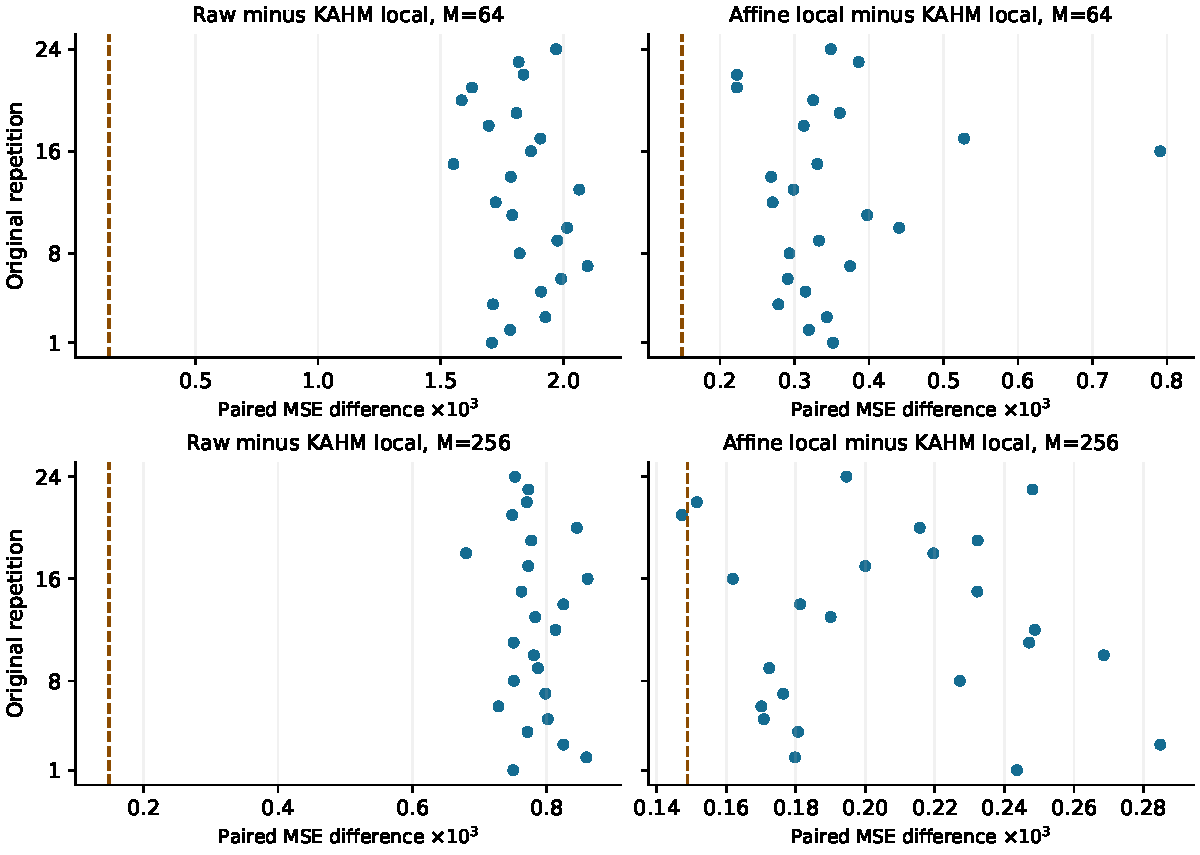
\includegraphics[width=.96\textwidth]{generated/figures/review_paired_differences.pdf}
\caption{The 24 original paired differences for each Van der Pol capacity comparison,
in units of $10^{-3}$ MSE. The dashed line is the frozen practical margin.
No resampling, refitting, or new primary analysis is performed.}
\label{fig:review-paired}
\end{figure}

We also inspect the 120 first-stage primary banks and 72 capacity banks from a
completed computational reproduction using the published seeds. No bank or head is
refitted for these diagnostics. Replayed test inputs, targets, and groups are checked
against their recorded hashes before the original feature map is evaluated.
Let $A$ vertically stack the $P_c^\top$ matrices. Proposition~\ref{prop:local-injectivity}
shows that positive gates and full column rank of $A$ suffice to recover the scaled
input from the gated local coordinates and gates:
division by $\phi_c$ recovers $P_c^\top(z-\mu_c)$, after which one solves for $z$.
A deficient stack does not establish information loss in the full code, because the
gates can carry additional information. Numerical ranks use the threshold
$\sigma_1\max\{\text{rows}(A),d\}\epsilon_{64}$; they are finite-precision diagnostics,
not exact rank proofs. Small singular values and small gates can make coordinate
recovery sensitive to perturbations. Test-sample gate minima are not population
lower bounds, and these computations do not guarantee a well-conditioned inverse
or easy decoding by any particular fitted head.
\begin{table}[htbp]
\caption{Retrospective diagnostics over 24 stored banks per row. Rank ranges concern
the stacked local bases in input dimension $d$. The smallest singular value and
gate entries are minima over the inspected banks (and, for gates, their original
test observations); $\kappa_2$ is the largest stack condition number. A dash means
that not every stack in that row has full numerical column rank. KAHM and affine
representations share the basis stack. Computational reproduction supplies no new
independent statistical replications.}
\label{tab:review-banks}
\centering\small\setlength{\tabcolsep}{3pt}
% Full column rank is sufficient; numerical ranks are diagnostics, not exact proofs.
\begin{tabular}{llrrrr}
\toprule
Phase / setting & Rank / $d$ & Min. $\sigma_d$ & Max. $\kappa_2$ & Min. $\phi^{\K}$ & Min. $\phi^{\A}$ \\
\midrule
First: Straight branch & 1/2 & $0$ & --- & $3.36\times10^{-25}$ & $2.56\times10^{-20}$ \\
First: Curved branch & 2/2 & $2.19\times10^{0}$ & $1.39\times10^{0}$ & $3.55\times10^{-28}$ & $8.97\times10^{-29}$ \\
First: Nonlinear AR & 12/12 & $6.20\times10^{-2}$ & $4.90\times10^{1}$ & $2.21\times10^{-35}$ & $2.36\times10^{-34}$ \\
First: Van der Pol & 12/12 & $1.60\times10^{-2}$ & $2.20\times10^{2}$ & $2.84\times10^{-45}$ & $9.43\times10^{-20}$ \\
First: Duffing & 12/12 & $1.33\times10^{-2}$ & $2.80\times10^{2}$ & $3.92\times10^{-43}$ & $3.11\times10^{-7}$ \\
Capacity: Nonlinear AR & 12/12 & $7.31\times10^{-2}$ & $4.19\times10^{1}$ & $9.97\times10^{-37}$ & $7.75\times10^{-37}$ \\
Capacity: Van der Pol & 12/12 & $1.60\times10^{-2}$ & $2.19\times10^{2}$ & $6.21\times10^{-44}$ & $1.56\times10^{-16}$ \\
Capacity: Duffing & 12/12 & $1.32\times10^{-2}$ & $2.84\times10^{2}$ & $5.38\times10^{-43}$ & $1.86\times10^{-8}$ \\
\bottomrule
\end{tabular}

\end{table}


\clearpage
\section{Additional Source-Derived Tables}\label{app:tables}

Tables~\ref{tab:reconstruction-details} and
\ref{tab:reflection-details} give descriptive input-geometry summaries.
The two complete primary comparison families follow. Their values
are generated from the archived outcomes, with each difference,
standard error, interval, and frozen margin independently recomputed
by the paper-asset script before it writes these tables.

\begin{table}[!htbp]
 \caption{Held-out reconstruction errors per standardized input coordinate,
 averaged over the three blocks and 24 full repetitions. ``Best'' takes
 the best local reconstruction separately in each block; ``weighted''
 averages the individual squared errors with that method's affinities.
 The affine value is lower in all 24 repetitions of each of these five
 input settings, for both summaries. These are descriptive diagnostics,
 not the supervised primary endpoint.}
 \label{tab:reconstruction-details}
 \centering\small\setlength{\tabcolsep}{4pt}
 % Generated by scripts/build_paper_assets.py; do not edit.
\begin{tabular}{lrrrr}
\toprule
Setting & KAHM best & Affine best & KAHM weighted & Affine weighted \\
\midrule
Branch $c=0$ & $3.276\times10^{-3}$ & $2.156\times10^{-16}$ & $4.006\times10^{-3}$ & $1.548\times10^{-8}$ \\
Branch $c=1$ & $3.583\times10^{-2}$ & $2.932\times10^{-2}$ & $3.793\times10^{-2}$ & $3.238\times10^{-2}$ \\
Nonlinear AR & $1.166\times10^{-2}$ & $1.084\times10^{-2}$ & $1.305\times10^{-2}$ & $1.214\times10^{-2}$ \\
Van der Pol & $4.353\times10^{-3}$ & $1.683\times10^{-3}$ & $4.495\times10^{-3}$ & $1.916\times10^{-3}$ \\
Duffing & $4.877\times10^{-3}$ & $5.613\times10^{-4}$ & $5.239\times10^{-3}$ & $1.226\times10^{-3}$ \\
\bottomrule
\end{tabular}

\end{table}

\begin{table}[!htbp]
 \caption{Branch reflection differences at training size 1,024, averaged
 over 24 banks. The statistic is a per-coordinate RMS, with and without
 training-only coordinate scaling. The raw reflection precedes the
 frozen pipeline. These values neither establish exact information
 loss for the learned code nor certify a decoder-specific population
 risk bound.}
 \label{tab:reflection-details}
 \centering\small\setlength{\tabcolsep}{5pt}
 % Generated by scripts/build_paper_assets.py; do not edit.
\begin{tabular}{rlrr}
\toprule
$c$ & Encoding & Stored-coordinate RMS & Standardized RMS \\
\midrule
0 & KAHM $\phi$ & $4.894\times10^{-1}$ & $1.402\times10^{0}$ \\
0 & Affine $\phi$ & $1.451\times10^{-9}$ & $7.533\times10^{-9}$ \\
0 & KAHM local & $5.289\times10^{-1}$ & $1.418\times10^{0}$ \\
0 & Affine local & $4.993\times10^{-1}$ & $1.236\times10^{0}$ \\
1 & KAHM $\phi$ & $5.380\times10^{-1}$ & $1.427\times10^{0}$ \\
1 & Affine $\phi$ & $5.321\times10^{-1}$ & $1.471\times10^{0}$ \\
1 & KAHM local & $4.854\times10^{-1}$ & $1.442\times10^{0}$ \\
1 & Affine local & $5.522\times10^{-1}$ & $1.473\times10^{0}$ \\
\bottomrule
\end{tabular}

\end{table}

\begin{table}[!htbp]
 \caption{Complete representation means in the fresh capacity study,
 with MSE multiplied by $10^3$. The full-score KAHM representation is
 a prespecified secondary control. These point estimates do not add
 hypotheses to the 12-comparison primary family.}
 \label{tab:capacity-means-details}
 \centering\small\setlength{\tabcolsep}{4pt}
 % Generated by scripts/build_paper_assets.py; do not edit.
\begin{tabular}{lrrrrr}
\toprule
System & $M$ & Raw & Affine local & KAHM local & KAHM scores \\
\midrule
Nonlinear AR & 64 & 4.4238 & 4.9120 & 4.8795 & 4.7984 \\
Nonlinear AR & 256 & 4.6958 & 5.2347 & 5.1749 & 4.8256 \\
Van der Pol & 64 & 2.8586 & 1.3767 & 1.0266 & 1.5711 \\
Van der Pol & 256 & 1.6541 & 1.0780 & 0.8720 & 1.0499 \\
Duffing & 64 & 3.4597 & 3.0549 & 4.2154 & 4.7005 \\
Duffing & 256 & 2.8364 & 2.7981 & 4.0736 & 3.3808 \\
\bottomrule
\end{tabular}

\end{table}

\clearpage
\subsection{Selected pipelines and realized dimensions}

The validation-selected pipeline and the retained nonlinear basis are
distinct summaries: the former describes the operational model choice,
whereas the latter records the realized dimensions behind the nominal
landmark budgets.

\begin{table}[!htbp]
 \caption{Secondary validation-only selection among the eight complete
 capacity-study pipelines. Mean test MSE is multiplied by $10^3$.
 Counts concern independent complete repetitions under each generator,
 not a new population of forecasting tasks.}
 \label{tab:capacity-selector-details}
 \centering\small\setlength{\tabcolsep}{4pt}
 % Generated by scripts/build_paper_assets.py; do not edit.
\begin{tabular}{lrl}
\toprule
System & Selector MSE & Validation selections \\
\midrule
Nonlinear AR & 4.4238 & Raw, 64: 24/24 \\
Van der Pol & 0.8720 & KAHM local, 256: 24/24 \\
Duffing & 2.7923 & Affine local, 256: 23/24; Raw, 256: 1/24 \\
\bottomrule
\end{tabular}

\end{table}

\begin{table}[!htbp]
 \caption{Retained RBF-plus-linear dimensions after the Nystr\"om
 eigenvalue cutoff in the fresh capacity study. Means and ranges cover
 the 24 repetitions in each cell. The same landmark count $M$ does not
 imply the same realized dimension or function class.}
 \label{tab:capacity-dimensions-details}
 \centering\small\setlength{\tabcolsep}{5pt}
 % Generated by scripts/build_paper_assets.py; do not edit.
\begin{tabular}{lrlrr}
\toprule
System & $M$ & Representation & Mean dimension & Range \\
\midrule
Nonlinear AR & 64 & Raw & 74.88 & 61--76 \\
Nonlinear AR & 64 & Affine local & 106.00 & 106--106 \\
Nonlinear AR & 64 & KAHM local & 106.00 & 106--106 \\
Nonlinear AR & 64 & KAHM scores & 76.71 & 62--78 \\
Nonlinear AR & 256 & Raw & 189.04 & 78--268 \\
Nonlinear AR & 256 & Affine local & 297.62 & 296--298 \\
Nonlinear AR & 256 & KAHM local & 297.50 & 293--298 \\
Nonlinear AR & 256 & KAHM scores & 148.88 & 77--219 \\
Van der Pol & 64 & Raw & 76.00 & 76--76 \\
Van der Pol & 64 & Affine local & 106.00 & 106--106 \\
Van der Pol & 64 & KAHM local & 106.00 & 106--106 \\
Van der Pol & 64 & KAHM scores & 78.00 & 78--78 \\
Van der Pol & 256 & Raw & 268.00 & 268--268 \\
Van der Pol & 256 & Affine local & 298.00 & 298--298 \\
Van der Pol & 256 & KAHM local & 272.38 & 261--285 \\
Van der Pol & 256 & KAHM scores & 231.88 & 215--251 \\
Duffing & 64 & Raw & 76.00 & 76--76 \\
Duffing & 64 & Affine local & 106.00 & 106--106 \\
Duffing & 64 & KAHM local & 105.46 & 98--106 \\
Duffing & 64 & KAHM scores & 77.96 & 77--78 \\
Duffing & 256 & Raw & 268.00 & 268--268 \\
Duffing & 256 & Affine local & 296.92 & 272--298 \\
Duffing & 256 & KAHM local & 240.38 & 176--298 \\
Duffing & 256 & KAHM scores & 214.33 & 164--270 \\
\bottomrule
\end{tabular}

\end{table}

\clearpage
% Generated; this file owns its longtable environment.
\begingroup\small\setlength{\tabcolsep}{3pt}
\begin{longtable}{llrrrl}
\caption{Complete first-stage family (29 contrasts), in original MSE units. Intervals use the two-sided 95\% Bonferroni paired-replicate Student procedure with 23 degrees of freedom. Under paired normality, each t interval is exact and Bonferroni family coverage is at least 95\%; otherwise coverage is approximate. The two stages have separate families.}\label{tab:all-stageone}\\
\toprule
Setting / budget & Contrast & $\overline D$ & Simultaneous interval & $\delta$ & Assessment \\
\midrule
\endfirsthead
\toprule
Setting / budget & Contrast & $\overline D$ & Simultaneous interval & $\delta$ & Assessment \\
\midrule
\endhead
\bottomrule\endfoot
$c=0,\lambda=0$ & $G$ & -0.000013 & $[-0.000031,\,0.000005]$ & 0.000168 & unresolved $\dagger$ \\
$c=0,\lambda=0$ & $N$ & -0.000008 & $[-0.000016,\,\ensuremath{-1.85\times10^{-7}}]$ & 0.000168 & negative $\dagger$ \\
$c=0,\lambda=0$ & $L$ & -0.000031 & $[-0.000043,\,-0.000020]$ & 0.000168 & negative $\dagger$ \\
$c=0,\lambda=0.5$ & $G$ & 0.489453 & $[0.481962,\,0.496944]$ & 0.000168 & practical + \\
$c=0,\lambda=0.5$ & $N$ & 0.000944 & $[0.000088,\,0.001799]$ & 0.000168 & positive \\
$c=0,\lambda=0.5$ & $L$ & 0.010616 & $[0.010033,\,0.011200]$ & 0.000168 & practical + \\
$c=0,\lambda=1$ & $G$ & 0.978026 & $[0.962552,\,0.993500]$ & 0.000168 & practical + \\
$c=0,\lambda=1$ & $N$ & 0.001938 & $[0.000255,\,0.003621]$ & 0.000168 & practical + \\
$c=0,\lambda=1$ & $L$ & 0.021287 & $[0.020199,\,0.022376]$ & 0.000168 & practical + \\
$c=1,\lambda=0$ & $G$ & 0.001761 & $[-0.071260,\,0.074781]$ & 0.033542 & unresolved \\
$c=1,\lambda=0$ & $N$ & 0.069128 & $[0.028663,\,0.109593]$ & 0.033542 & positive \\
$c=1,\lambda=0$ & $L$ & 0.263144 & $[0.217187,\,0.309101]$ & 0.033542 & practical + \\
$c=1,\lambda=0.5$ & $G$ & -0.004395 & $[-0.043672,\,0.034882]$ & 0.016863 & unresolved \\
$c=1,\lambda=0.5$ & $N$ & 0.040663 & $[0.019789,\,0.061538]$ & 0.016863 & practical + \\
$c=1,\lambda=0.5$ & $L$ & 0.154710 & $[0.122867,\,0.186552]$ & 0.016863 & practical + \\
$c=1,\lambda=1$ & $G$ & 0.011324 & $[0.000882,\,0.021767]$ & 0.000168 & practical + \\
$c=1,\lambda=1$ & $N$ & 0.012111 & $[0.005647,\,0.018574]$ & 0.000168 & practical + \\
$c=1,\lambda=1$ & $L$ & 0.046854 & $[0.040400,\,0.053307]$ & 0.000168 & practical + \\
Nonlinear AR & $G$ & \ensuremath{-1.89\times10^{-7}} & $[-0.000050,\,0.000049]$ & 0.000253 & unresolved $\dagger$ \\
Nonlinear AR & $N$ & -0.000016 & $[-0.000062,\,0.000029]$ & 0.000253 & unresolved $\dagger$ \\
Nonlinear AR & $L$ & 0.000433 & $[0.000368,\,0.000498]$ & 0.000253 & practical + \\
Van der Pol & $G$ & -0.049419 & $[-0.060532,\,-0.038307]$ & 0.002036 & negative \\
Van der Pol & $N$ & 0.013443 & $[0.005084,\,0.021803]$ & 0.002036 & practical + \\
Van der Pol & $L$ & 0.096633 & $[0.092436,\,0.100830]$ & 0.002036 & practical + \\
Duffing & $G$ & -0.030948 & $[-0.035414,\,-0.026482]$ & 0.000338 & negative \\
Duffing & $N$ & 0.005558 & $[0.001721,\,0.009395]$ & 0.000338 & practical + \\
Duffing & $L$ & 0.046168 & $[0.041729,\,0.050608]$ & 0.000338 & practical + \\
$c=0$ interaction & $I_0$ & -0.978039 & $[-0.993512,\,-0.962566]$ & 0.000168 & opposite sign \\
$c=1$ interaction & $I_1$ & -0.009564 & $[-0.082839,\,0.063712]$ & 0.016855 & unresolved \\
\end{longtable}
\noindent $\dagger$: the entire interval lies within the fixed practical band $[-\delta,\delta]$. An unresolved sign alone does not establish equivalence.
\endgroup

\clearpage
% Generated; this file owns its longtable environment.
\begingroup\small\setlength{\tabcolsep}{3pt}
\begin{longtable}{llrrrl}
\caption{Complete fresh capacity family (12 contrasts). All numerical loss quantities are multiplied by $10^3$. Intervals use the two-sided 95\% Bonferroni paired-replicate Student procedure with 23 degrees of freedom. Under paired normality, each t interval is exact and Bonferroni family coverage is at least 95\%; otherwise coverage is approximate. The two stages have separate families.}\label{tab:all-capacity}\\
\toprule
Setting / budget & Contrast & $\overline D$ & Simultaneous interval & $\delta$ & Assessment \\
\midrule
\endfirsthead
\toprule
Setting / budget & Contrast & $\overline D$ & Simultaneous interval & $\delta$ & Assessment \\
\midrule
\endhead
\bottomrule\endfoot
Nonlinear AR / 64 & Raw--K & -0.4556 & $[-0.5235,\,-0.3878]$ & 0.2201 & negative \\
Nonlinear AR / 64 & Affine--K & 0.0325 & $[-0.0031,\,0.0680]$ & 0.2201 & unresolved $\dagger$ \\
Nonlinear AR / 256 & Raw--K & -0.4791 & $[-0.6013,\,-0.3569]$ & 0.2201 & negative \\
Nonlinear AR / 256 & Affine--K & 0.0598 & $[-0.0131,\,0.1327]$ & 0.2201 & unresolved $\dagger$ \\
Van der Pol / 64 & Raw--K & 1.8320 & $[1.7369,\,1.9271]$ & 0.1489 & practical + \\
Van der Pol / 64 & Affine--K & 0.3501 & $[0.2755,\,0.4247]$ & 0.1489 & practical + \\
Van der Pol / 256 & Raw--K & 0.7822 & $[0.7550,\,0.8094]$ & 0.1489 & practical + \\
Van der Pol / 256 & Affine--K & 0.2060 & $[0.1810,\,0.2311]$ & 0.1489 & practical + \\
Duffing / 64 & Raw--K & -0.7557 & $[-1.0831,\,-0.4282]$ & 0.1727 & negative \\
Duffing / 64 & Affine--K & -1.1605 & $[-1.4707,\,-0.8503]$ & 0.1727 & negative \\
Duffing / 256 & Raw--K & -1.2372 & $[-1.5242,\,-0.9503]$ & 0.1727 & negative \\
Duffing / 256 & Affine--K & -1.2756 & $[-1.5702,\,-0.9810]$ & 0.1727 & negative \\
\end{longtable}
\noindent $\dagger$: the entire interval lies within the fixed practical band $[-\delta,\delta]$. An unresolved sign alone does not establish equivalence.
\endgroup


\end{document}
